\chapter{Implementation and Experiments} \label{implementation}

In this chapter, we describe our the implementations of our algorithms along with the experimental results obtained. In Section \ref{dataSets} we give detailed descriptions of all the data sets we have generated. Section \ref{costfns} describes all the cost functions we have used for our experiments. Section \ref{impldet} gives specific details about the programming language and underlying data structures used for our implementations. In Section \ref{hypothesis} we list the hypothesis that we expect to verify with our experiments and present experimental results in Section \ref{experiments}. 

\section{Data Sets} \label{dataSets}
We generate input sequences of sizes 100, 1000, 10,000 and 100,000. Each input item in the sequence is assigned a colour within the range 1 \ldots $C$. In order to recommend algorithms for various application scenarios we generate data sets that follow a specific pattern as well as random data sets. We have performed experiments on the following data sets for all our algorithms for different size combinations of the input parameters.

\begin{itemize}
\item \textit{Random Sequence}: The colours for the input items are generated randomly between the range 1 \ldots $C$ with equal probability. An example of a random sequence with 3 colours and input size 10 is as follows: 3, 2, 3, 1, 2, 3, 2, 1, 1, 2. 
\item \textit{Sequential Block Sequence}: We use the notation $m$ to denote the block size. We assign a colour $c$, chosen from the range 1 \ldots $C$ to all input item belonging to the same block. We have assigned colours to each block, starting from the first block, in an increasing order from 1 going up to $C$. We repeat the same pattern of colours for the entire size of the input sequence. For our experiments we have used a block size of 5. An example of the sequence for block size 3, 2 colours and input sequence size 10 is as follows: 1, 1, 1, 2, 2, 2, 1, 1, 1, 2. 
\item \textit{Random Block Sequence}: In this case, we have a block sequence where the size of the blocks are randomly chosen within the range 1 \ldots $C$ and this randomly chosen size also corresponds to the colour assigned to each item in that particular block. An example of this sequence for input size 10 and 3 colours is as follows: 3, 3, 3, 1, 2, 2, 1, 1, 2, 2. For this example, 
\item \textit{Alternation Sequence}: In the alternation sequence, we generate the first item with colour $c$ and assign the colours $c + 1$, $c + 2$ \ldots $C$ for each successive item. For the sake of simplicity we have assigned  colours in the increasing order of the set of colours starting from 1. We repeat the same pattern until the end of the input sequence. An example of the sequence for 3 colours and input sequence size 10 is as follows: 1, 2, 3, 1, 2, 3, 1, 2, 3, 1. 
\item \textit{Delta Sequence}: In the delta sequence we generate input items that are always within a certain range. We use the notation $\Delta$ to denote this range. For this sequence, we generate the first item $c$ randomly within the range 1 \ldots $C$ and starting with the second item, we generate each item in the range of $c \pm \Delta$, where $\Delta$ can take the value 0. This ensures that all the items are within the range of $\Delta$ from the previous item. An example of the sequence for $\Delta$ value 2, 3 colours and input sequence size 10 is as follows: 2, 3, 1, 2, 2, 3, 1, 1, 2, 3. 
\end{itemize}

\section{Cost Functions} \label{costfns}

Since some of our algorithms are designed for the non-uniform cost model, we have designed the following cost functions and tested them with all the data sets listed in \ref{dataSets} to recommend algorithms for specific application scenarios. Our implementations are designed based on the assumption that we always consider the cost of the colour to which we are switching to, or the next \textit{new active output colour}. Our cost functions are as defined below:

\begin{itemize}
\item \textit{Uniform Cost}: In this case the cost assigned to every colour is uniform. For the sake of simplicity we have assumed a unit cost model for our uniform cost function. 
\item \textit{Cost Equals Colour}: For this cost model, the cost assigned to the colour is the value of the colour itself, for example, an item with colour 3 has a cost of 3.
\item \textit{Cost Equals Quadratic Colour}: In this case, the cost assigned to the colour is equal to the square of the value of the colour, for example, the cost of colour 3 is set to be 9. The reason behind having such a cost function is to examine our algorithms' performance when subject to input sequences where the cost of switching is very high and varies between very low and very high costs. 
\item \textit{Random Cost}: In this case we randomly assign a cost to each colour between the range 1 \ldots $R$. For our experiments we have set $R$ to be 5. The reason behind this is to limit the cost assigned to colours to be a low cost and compare our algorithms' performance when the cost of the colours in the input sequence is low.
\item \textit{Colour Difference Cost Function}: This is the only cost model that takes into account the colour that we are presently at, and the colour to which we would like to switch to. We call these two colours the \textit{from colour} and \textit{to colour}.  Here the cost of switching from the \textit{from colour} to the \textit{to colour} is defined as the absolute difference between the two colours. This cost model is especially applicable in scenarios where the cost of switching depends on the two colours in question. An application of this cost model can be seen in the disk scheduling problem where switching is synonymous to moving the disk head to point to a particular disk block. In this case we want to minimize the distance between moving the head too far from the current point. 
\end{itemize}

\section{Implementation Details} \label{impldet}
In this section we describe the assumptions made in our implementations and give a basic overview of our approach to the different algorithms we have implemented. Table \ref{implalgo} lists all the algorithms that we have implemented along with the size of the input sequences, buffer sizes and number of colours. We have performed experiments with different data sets (refer to Section \ref{dataSets}). \\

We have primarily used Java with the JavaSE-1.7 as our execution environment for most of our implementations. The native C GNU Linear Programming Kit (GLPK Simplex Optimizer), version v4.52 is used for the Linear Program that we have chosen to implement. Experimental results are presented in Section \ref{experiments}.

\begin{table}[ht]
\label{implalgo}
\caption{Algorithms implemented along with parameter values}
\centering
\begin{tabular}{l llll llll llll}
\hline \hline
Algorithm&\multicolumn{4}{l}{Input Sequence Size $N$}&\multicolumn{4}{l}{Buffer
Size $k$}&\multicolumn{4}{l}{Colours $C$} \\
\hline
Bounded Waste & 100 & 1000 & 10000 & 100000 & 2 & 10 & 50 & 100 & 2 & 10 & 50 &
100 \\
Maximum Adjusted Penalty & 100 & 1000 & 10000 & 100000 & 2 & 10 & 50 & 100 & 2 &
10 & 50 & 100 \\
Random Choice & 100 & 1000 & 10000 & 100000 & 2 & 10 & 50 & 100 & 2 & 10 & 50 &
100 \\
Round Robin & 100 & 1000 & 10000 & 100000 & 2 & 10 & 50 & 100 & 2 & 10 & 50 &
100 \\
Threshold or Lowest Cost & 100 & 1000 & 10000 & 100000 & 2 & 10 & 50 & 100 & 2 &
10 & 50 & 100 \\
Optimal Offline LP & 100 & 500 & - & - & 2 & 10 & 50 & 100 & 2 & 10 &
50 & 100 \\
New Algorithm & 100 & 1000 & 10000 & 100000 & 2 & 10 & 50 & 100 & 2 &
10 & 50 & 100 \\
\hline
\end{tabular}
\end{table}

Our input/output sequences and buffers are implemented as Java Array Lists. We build our input sequences according to the data sets listed in \ref{dataSets} by adding an item at the end of the list. Our algorithms also construct the output sequence in a similar manner by appending items to the end of the list. The main intuition behind using array lists for implementing our sequences and buffers is because it has the property of random access which how our algorithms specify the buffers. 

Every item is designed to have the colour, the input time which we set at the time of creation, the output time which specifies the time at which the item was evicted from the buffer and an optional counter which is specific to the algorithm. We begin our input time stamps from 1 and check to ensure that every item has an output time that is greater than the time at which it was input.

We define all the statistics that we would like to measure about our algorithms' performance on the sequences, and compare the input and output sequences to decide the proportion of switches that have been reduced, the proportion of switching cost that has been reduced, the minimum, maximum and the average time that an item spends in the buffer. 

Our basic outline for the reordering buffers happens in three stages: \textit{initialization}, \textit{reordering} and \textit{eviction}. In the \textit{initialization} phase, we fill the first $k$ items of the input sequence into the buffer. In the \textit{reordering} phase we first pick a new colour to evict from the different colours presently in the buffer, which we call as the \textit{new active colour} and evict one item of this colour in each time step. We then set the output time on the evicted item, add the item to the output sequence and refill the buffer. We continue to do this until all the input items are in the buffer have been processed by the buffer. In the \textit{eviction} phase, we empty the buffer and start evicting one item at each step until the buffer is empty. We also set output times and add the item to the output sequence as in the \textit{reordering} phase.

Our assumptions for individual algorithms and implementation details are as follows: 

\begin{itemize}
\item \textit{Bounded Waste}: Our outline for Bounded Waste differs from the other algorithms, in that when we have chosen the colour that we would like to evict from the buffer, we evict all the items of that colour in one step as opposed to one in each step. This causes many successive items to have the same output time, and we expect that the average time that an item spends in the buffer will also be reduced as a consequence of this. Our implementation follows our understanding of Bounded Waste as explained in Section \ref{bw}. 
\item \textit{Maximum Adjusted Penalty}
\item \textit{Random Choice}: As explained in Section \ref{rc}, we randomly select a colour present in the buffer and remove one item of that colour in each step, until there are no more items of that colour in the buffer. To choose a new active output colour, we randomly select a colour present in the buffer and continue until the input sequence has been processed and the buffer is empty. 
\item \textit{Round Robin}: For the Round Robin reordering, we initially set the selection pointer to point to the first item in the buffer, which is at index 0. When we have to choose a new active colour, we select the colour pointed to by the selection pointer in the buffer and remove one item of that colour at each step. But since our array list implementation of the buffer compresses the buffer to the left when an item is evicted, it skips a colour and moves to the next colour. We continue to do this until the input sequence has been processed and our buffer is empty.
\item \textit{Threshold or Lowest Cost} \ref{tlc}
\item \textit{New Algorithm} \ref{weird}
\item \textit{Optimal Offline LP}: The problem definition for the linear program is as specified in \cite{adamaszek2012optimal} and we have used the GNU Simplex Optimizer and C implementations to generate data sets and matrices for the linear program. 
\end{itemize}

\section{Hypothesis} \label{hypothesis}

\subsection{Input Sequence Size}

\hypothesis{For relatively small input sequence sizes, with a small buffer and a small number of colours, we expect that almost all of our algorithms will achieve approximately the same number of switches in the output sequence for both uniform and non-uniform costs.}

\hypothesis{For relatively small input sequences with a small buffer and a large number of colours we expect that there will not be any significant reordering, so the output sequence will have as many switches as the input sequence.}

We also expect that for very small input sequences, the re-ordering done by many of the algorithms will be the same, regardless of their competitive ratios. 

\hypothesis{For relatively small input sizes, with a large buffer and few colours, we expect that our algorithms will perform very well and have the same number of switches as the optimal offline algorithm.} 

\hypothesis{For relatively small input sizes, with a large buffer and a large number of colours, we expect that our algorithms will perform poorly. Even though the size of the buffer is relatively large, the small input sequence size combined with many colours would make re-ordering inefficient.}

\hypothesis{For very large input sequence sizes, with a small buffer and a small number of colours, we expect that our algorithms will achieve the claimed competitive ratios if the number of colours is less than the buffer size.}

\hypothesis{For very large input sequence sizes, with a small buffer and a large number of colours, we expect that there will not be any significant re-ordering as the buffer will most likely have items of different colours than the chosen output colour.}

\hypothesis{For very large input sequence sizes, with a large buffer and a small number of colours, we expect that our algorithms will achieve a very good performance with very few switches in the output sequence.} 

\hypothesis{For a very large input sequence, with a large buffer and a large number of colours, we expect that the algorithms will achieve a good performance if the number of colours is less than the buffer size.}

\subsection{Data Sets}
\hypothesis{We expect that all of our algorithms will do relatively well for the random sequences for large data sets and achieve the competitive ratios as claimed in the paper.}

\hypothesis{Reordering on block input sequences can be achieved if the buffer size is at least the size of the block size times the number of colours ($k = m * C$).}

\hypothesis{For small block sequences we expect that there will not be any significant reordering because of the small buffer size.}

\hypothesis{We expect the alternation sequences to achieve a good competitive ratio if for large input sizes if the buffer size is much greater than the number of colours.}

\hypothesis{For small input sequences with a small buffer reordering for alternation sequences will be minimal.}

\hypothesis{We expect that there will be efficient reordering for the delta sequences when the range is small, that is we have a small delta value and a large buffer.} 

\subsection{Uniform Costs}
\hypothesis{We expect that the number of switches between the output and the input sequences for the algorithms BW and MAP will be approximately the same.}

\hypothesis{We expect that the competitive ratio of BW and MAP for uniform costs will approximately be of the order of $O(\log k)$.}

\subsection{Non-Uniform Costs}
some more hypothesis have to be written here. write a more concise list of hypothesis for the others and cover the rest with small scale experiments. hypothesis on how algorithms perform with uniform costs as opposed to non-uniform costs.

\section{Experiments and Results} \label{experiments}
Section \ref{impldet} details all the algorithms we have implemented, along with the details of the implementation, our assumptions for the algorithms and language and programming details. We have performed different experiments on these algorithms for the all the data sets listed in Section \ref{dataSets} and all cost functions listed in Section \ref{costfns} to gain some insight to designing a new algorithm. These results are listed in the following subsections. 

Table \ref{implalgo} lists all our algorithms, along with the different sizes used for different input parameters. Experiments are performed once for each deterministic algorithm. For randomized algorithms with random data sets and random cost functions, we repeat the experiments 100 times and average the results from all experiments.\footnote{We have used Excel 2010 to analyze all our results and used Excel Pivot Tables to compute averages and plot charts for our experiments.} 

For each of our experiments, we record the following values: the algorithm that is being executed, the kind of input sequence used, the cost function, the size of the input sequence, the buffer size, number of colours, count of switches in the input sequence, count of switches in the output sequence, ratio of the output/input sequence switches count, cost of the input sequence, cost of the output sequence and the ratio of the output/input sequence cost. We use these ratios to plot our charts since it gives us an insight into how each algorithm performs under different data sets/ cost function combinations. The ratios gives us some insight into the percentage of how many switches were eliminated or how much of the cost was reduced. For example, let us assume that our input sequence has a size of 10, and has 8 switches in the input and 3 switches in the output, our ratio is 3/8 = 0.375. This indicates that the output sequence has 37.5\% of the switches present in the input sequence. We use similar ratios to analyze the cost as well.

Our experimental results reveal that the lengths of the input sequences do not play a significant role in the way our algorithms perform with different buffer sizes, varied number of colours or even different data sets and cost functions. We briefly explain our results as seen with the input sequences and show some graphs to infer that the performance of our algorithms' does not depend on the size of the input sequence.

For Random Sequences with a Uniform Cost Function, we observe that the ratio of the Output/Input cost stays the same for all input sequence sizes, meaning that regardless of the input sequence size, the reordering is only dependent on the buffer size and number of colours. This has been observed across all algorithms for all input sizes as illustrated in Figure \ref{lengthsRandomSeqUniformCost}. Similar results have been seen for all the other kinds of input sequences for the Uniform Cost Function. 

\begin{figure}[ht]
\centering 
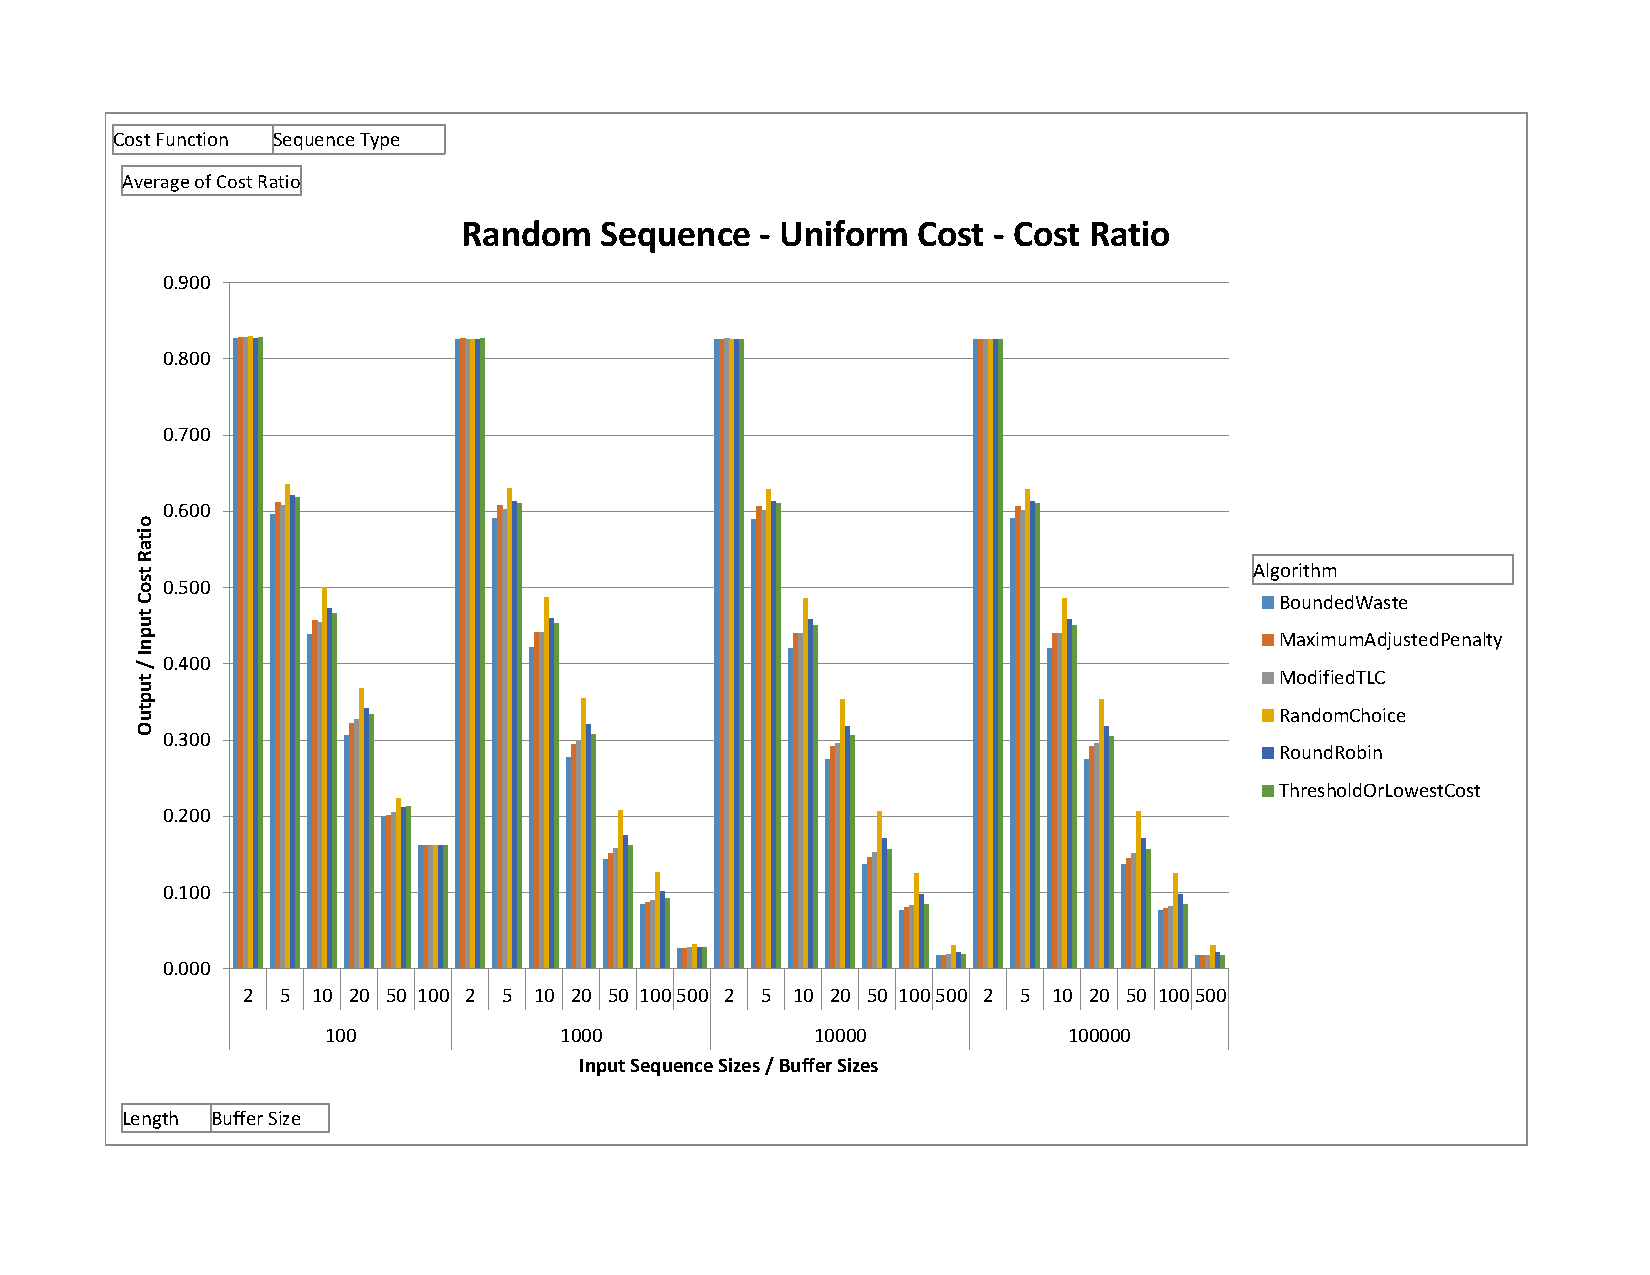
\includegraphics[scale=0.60]{Lenghts-Random-Seq-Uniform-Cost.pdf}
\caption{Random-Sequence-Uniform-Cost}
\label{lengthsRandomSeqUniformCost}
\end{figure}

While different algorithms have different performance for different combinations of data sets and cost functions, the general trend suggests that they do not heavily depend on the size of the input sequence. This has been true in the case of all kinds of data sets when subjected to the Cost Equals Colour Cost Function and Cost Equals Quadratic Colour as well. 

For the Sequential Block Sequence with a Cost Equals Colour Difference Cost Function, we see that the Random Choice and the Round Robin algorithms achieve the worst performance in general and specifically for input size 100. As seen in other cases the size of the input sequence is insignificant in the reordering that can be achieved by the algorithm. This is illustrated in Figure \ref{lengthsSequentialBlockSeqColourDifference}. 

\begin{figure}[ht]
\centering 
%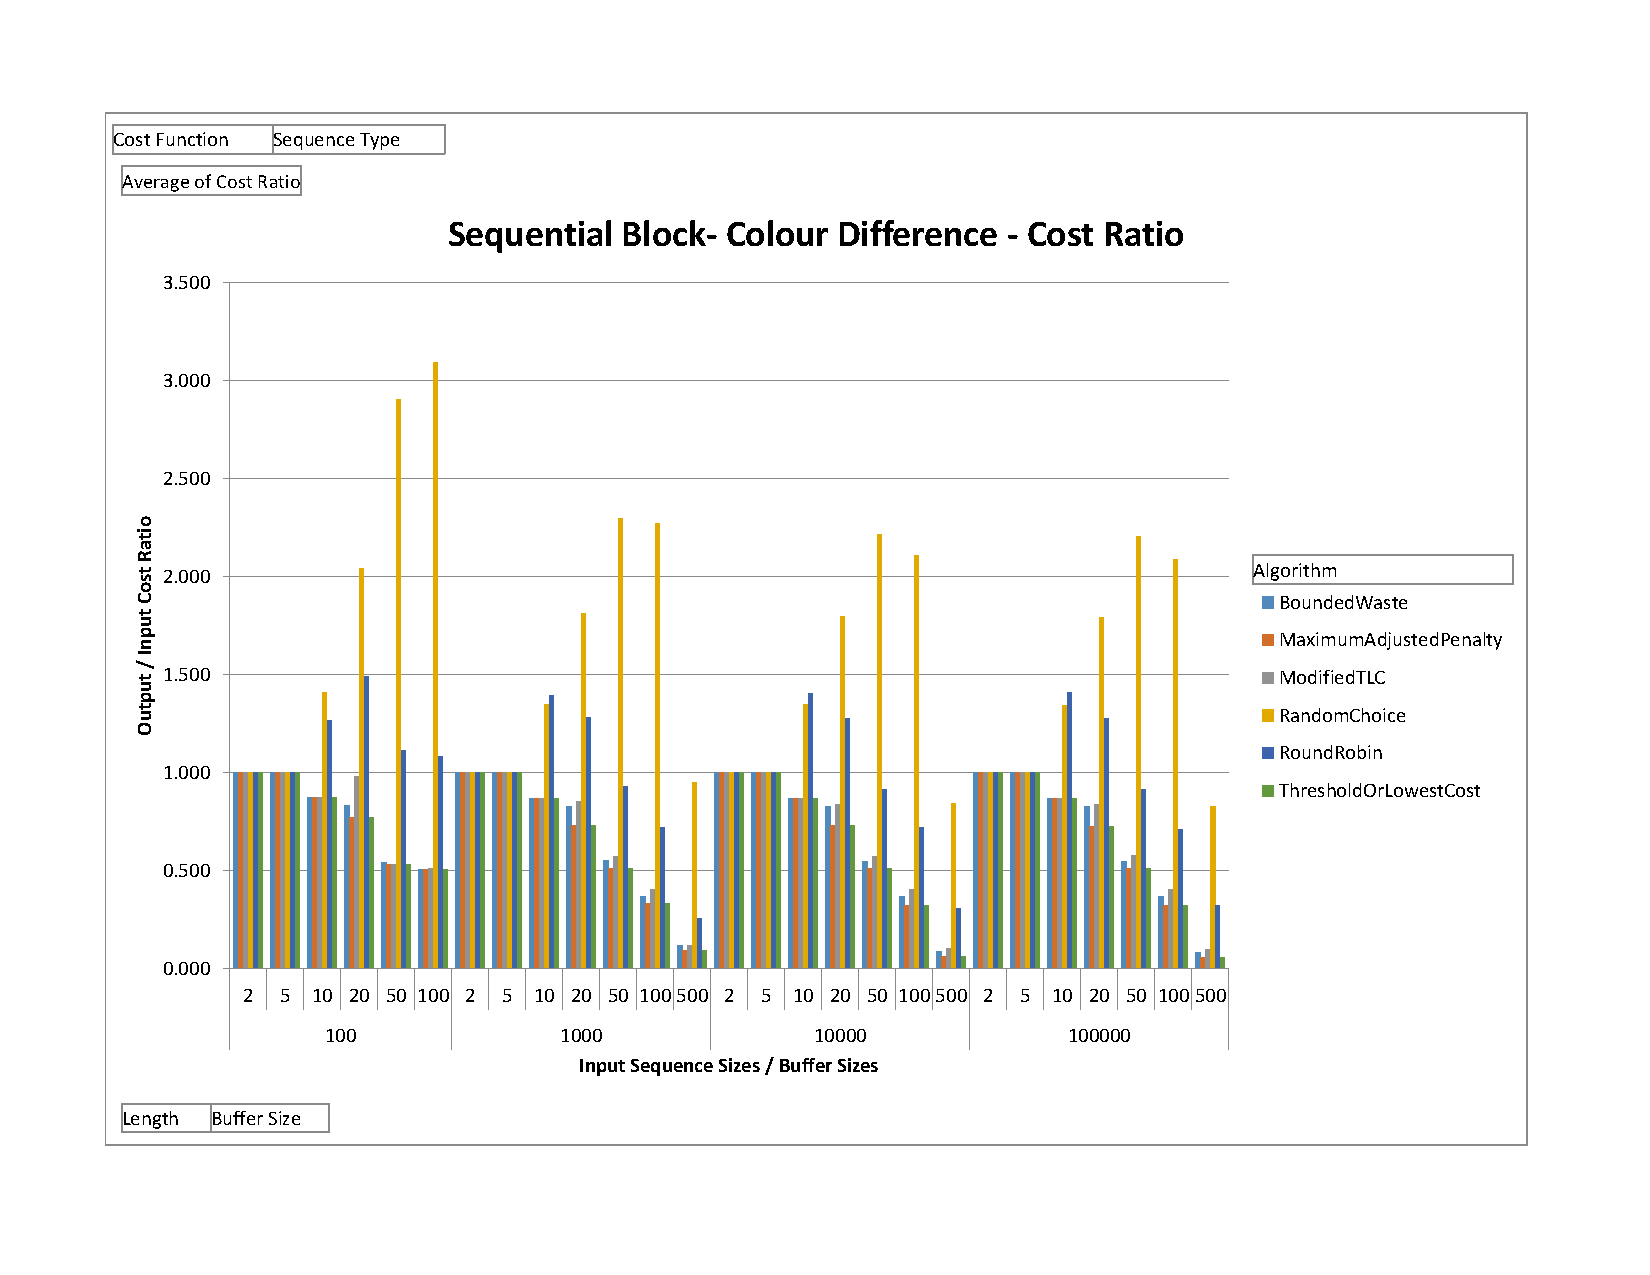
\includegraphics[trim=20mm 25mm 20mm 20mm,clip,width=0.90\columnwidth]{Lengths-Sequential-Block-Colour-Difference.pdf}
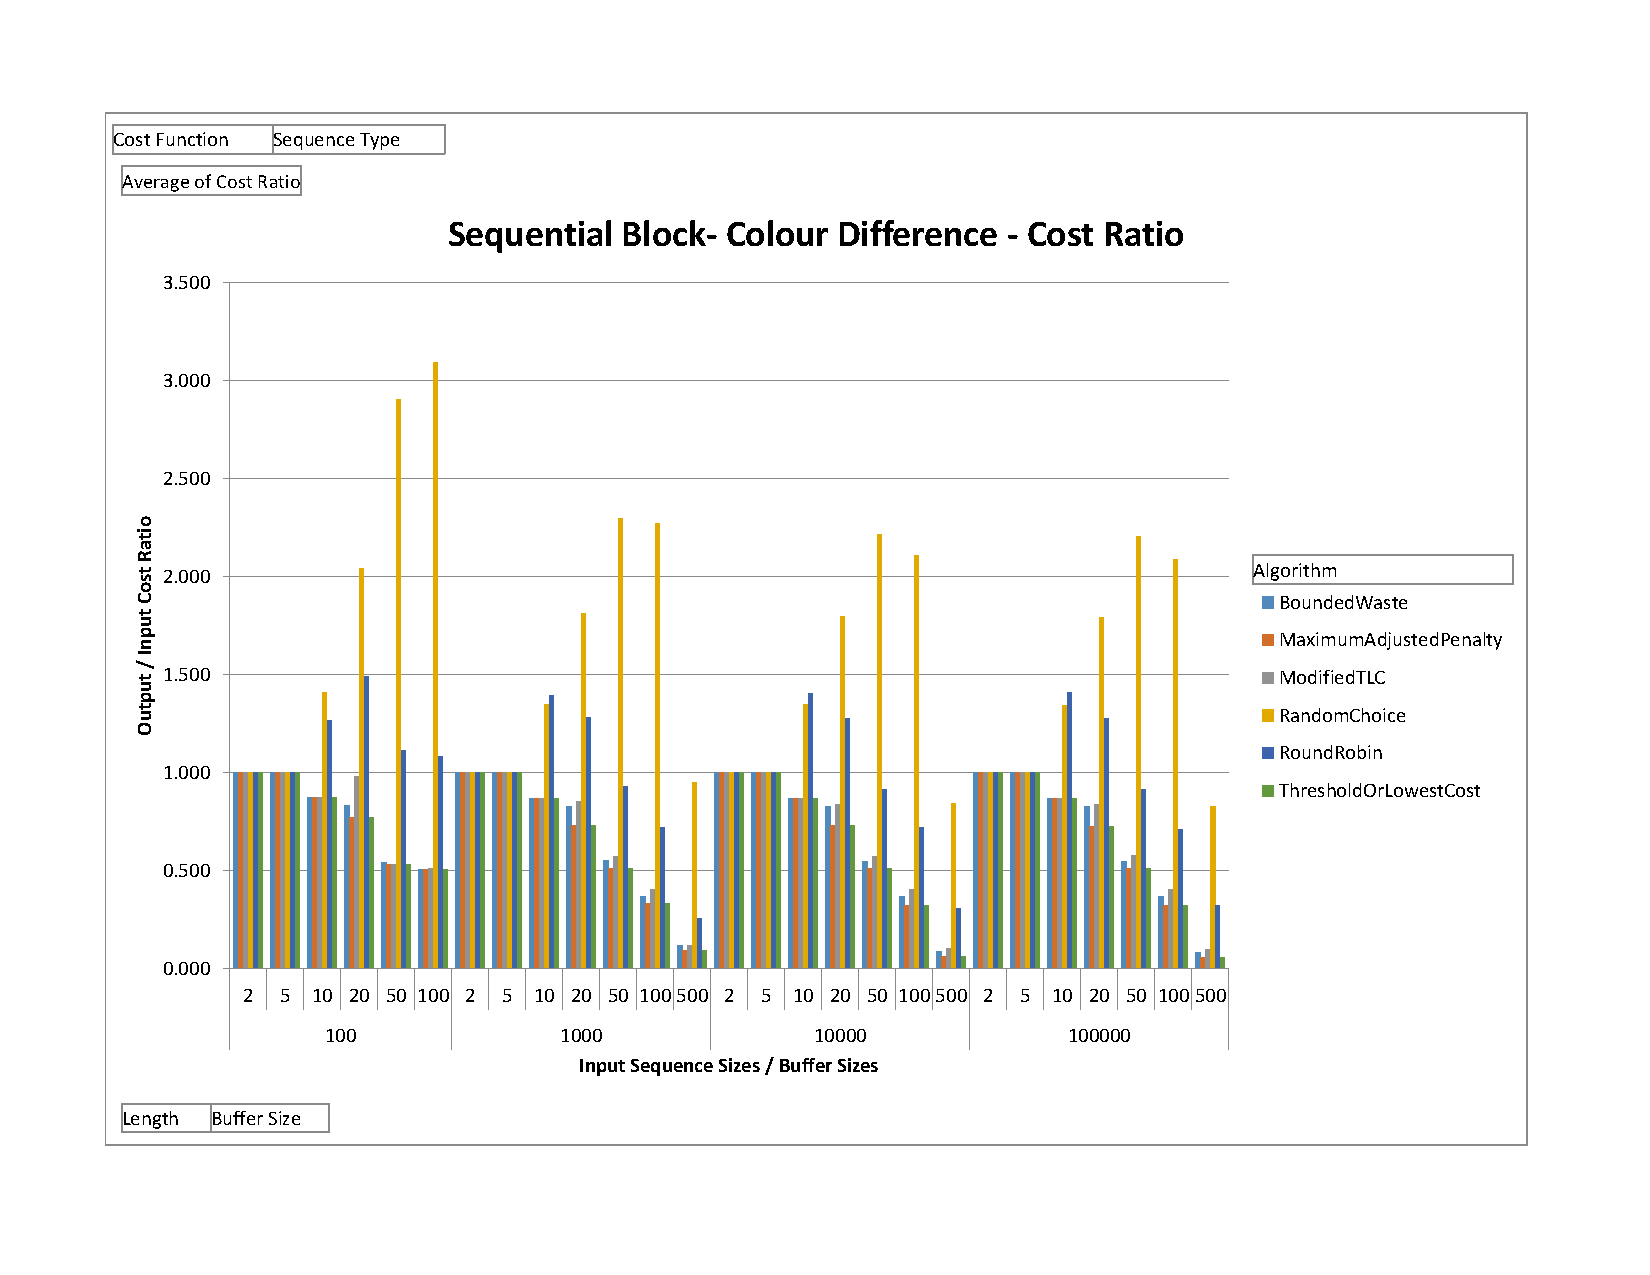
\includegraphics[scale=0.60]{Lengths-Sequential-Block-Colour-Difference.pdf}
\caption{Sequential-Block-Colour-Difference-Cost}
\label{lengthsSequentialBlockSeqColourDifference}
\end{figure}

We describe how different algorithms perform with the different data sets and cost function combinations in the following subsections and supplement them with appropriate figures.

\subsection{Alternation Sequences}

Alternation Sequences with a Uniform Cost model have no reordering when the number of colours is greater than the buffer size. As a result we see little or no reordering for buffer sizes 2, 5 and 10 across all algorithms. One would expect this behaviour since the alternation sequence switches colour on every input item and with a small buffer, it is likely that each item in the buffer has a different colour forcing the algorithm to make a colour change. For larger buffer sizes (50, 100 and 500) we notice that most of our algorithms achieve the same performance with only marginal difference in the Output/Input cost ratio. Our exceptions are the Random Choice and Round Robin algorithms which do not perform as well as the deterministic algorithms. We believe that this might be due to the randomness introduced by the algorithms, and that the algorithm might be selecting colours that only have a few occurrences in the buffer causing the algorithm to make another switch. 

For the Cost Equals Colour model, TLC performs slightly better when the buffer sizes are very small. ModifiedTLC and MAP fail to perform any reordering in this case. But as the buffer sizes increase, MAP and ModifiedTLC achieve a much better performance than TLC with ModifiedTLC only having 6.2\% of the switches present in the input sequence when the buffer size is 500 and the input sequence has 50 colours. This is illustrated in Figure\ref{AlternationSeqCostEqualsColourSwitches}. ModifiedTLC and MAP do not achieve a good reordering when the buffer size is less than the number of colours, however, TLC does achieve minimal reordering in this case. 

\begin{figure}[ht]
\centering 
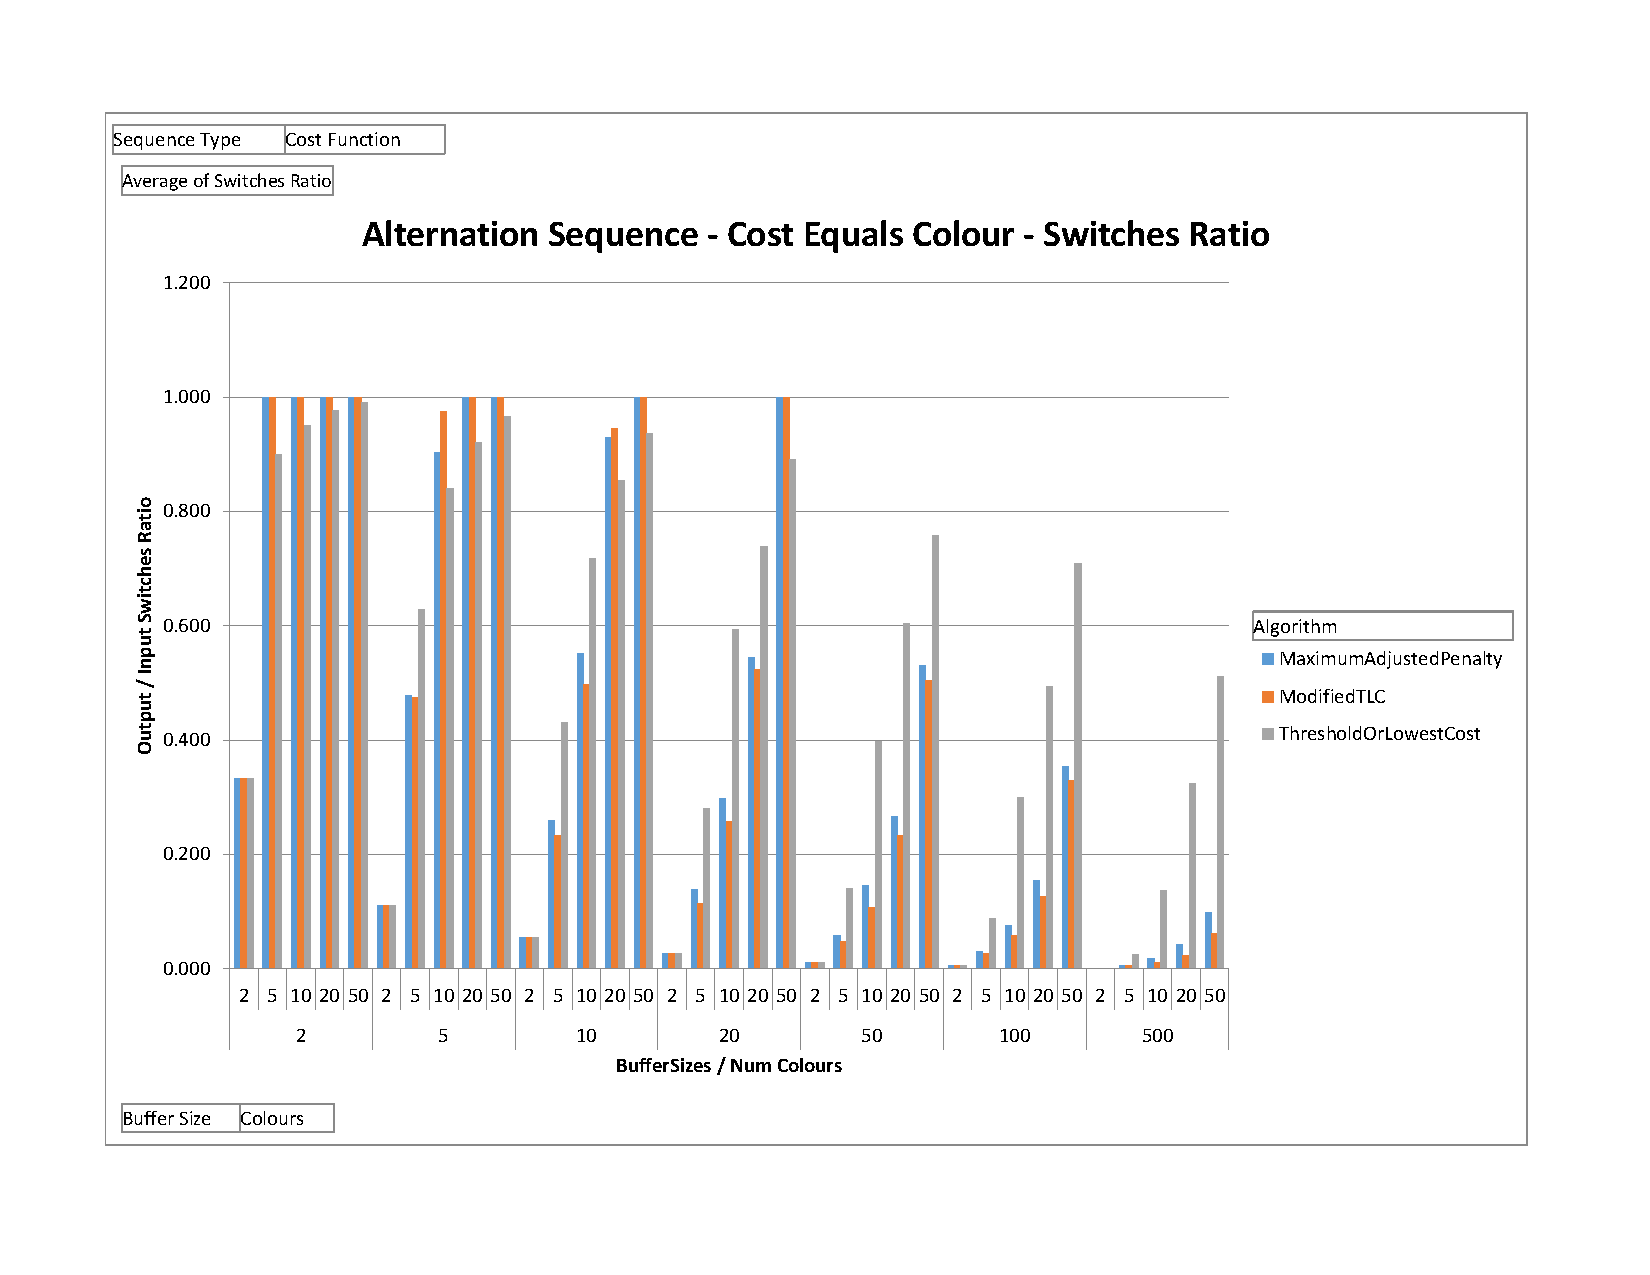
\includegraphics[scale=0.60]{Alternation-Seq-Cost-Equals-Colour-Switches.pdf}
\caption{Alternation-Sequence-Cost-Equals-Colour-Switches-Ratio: ModifiedTLC performs better than MAP and TLC}
\label{AlternationSeqCostEqualsColourSwitches}
\end{figure}

We observe the same behaviour for the Cost Equals Quadratic Colour cost model where TLC performs marginally better when the buffer sizes are small, but for larger buffer sizes (50, 100 and 500) ModifiedTLC outperforms TLC by a great extent, having only 35.6\% of switches present in the input sequence and has only 9\% of the switches present in the input sequence for 50 colours. Similar results also hold good for costs where ModifiedTLC only has 24.5\% of the cost of the input sequence, having only 4.6\% of the cost for a buffer size of 500 and 50 input colours. ModifiedTLC also performs better than MAP in this case. 

Random Cost models also exhibit similar behaviour, with TLC achieving a better performance with small buffers and MAP and ModifiedTLC achieving a good performance for large buffers. MAP and ModifiedTLC only achieve minimal reordering when the buffer size is less than the number of colours. They do better only for buffer sizes 50, 100 and 500. 

The Colour Difference cost model shows some interesting results for Alternation Sequences. It is interesting to note that all our algorithms fail to reorder the input sequence when the number of colours is greater than the buffer size. Another point of interest is that MAP and TLC perform exactly the same across all buffer sizes and number of colours, and ModifiedTLC marginally performs better than the two w.r.t reducing the number of switches in the input sequence as illustrated in chart \ref{AlternationSeqColourDifferenceSwitches}. This behaviour is also exactly the same w.r.t the cost except that ModifiedTLC is not as cost efficient as MAP or TLC. (figure out why this happens)

\begin{figure}[ht]
\centering 
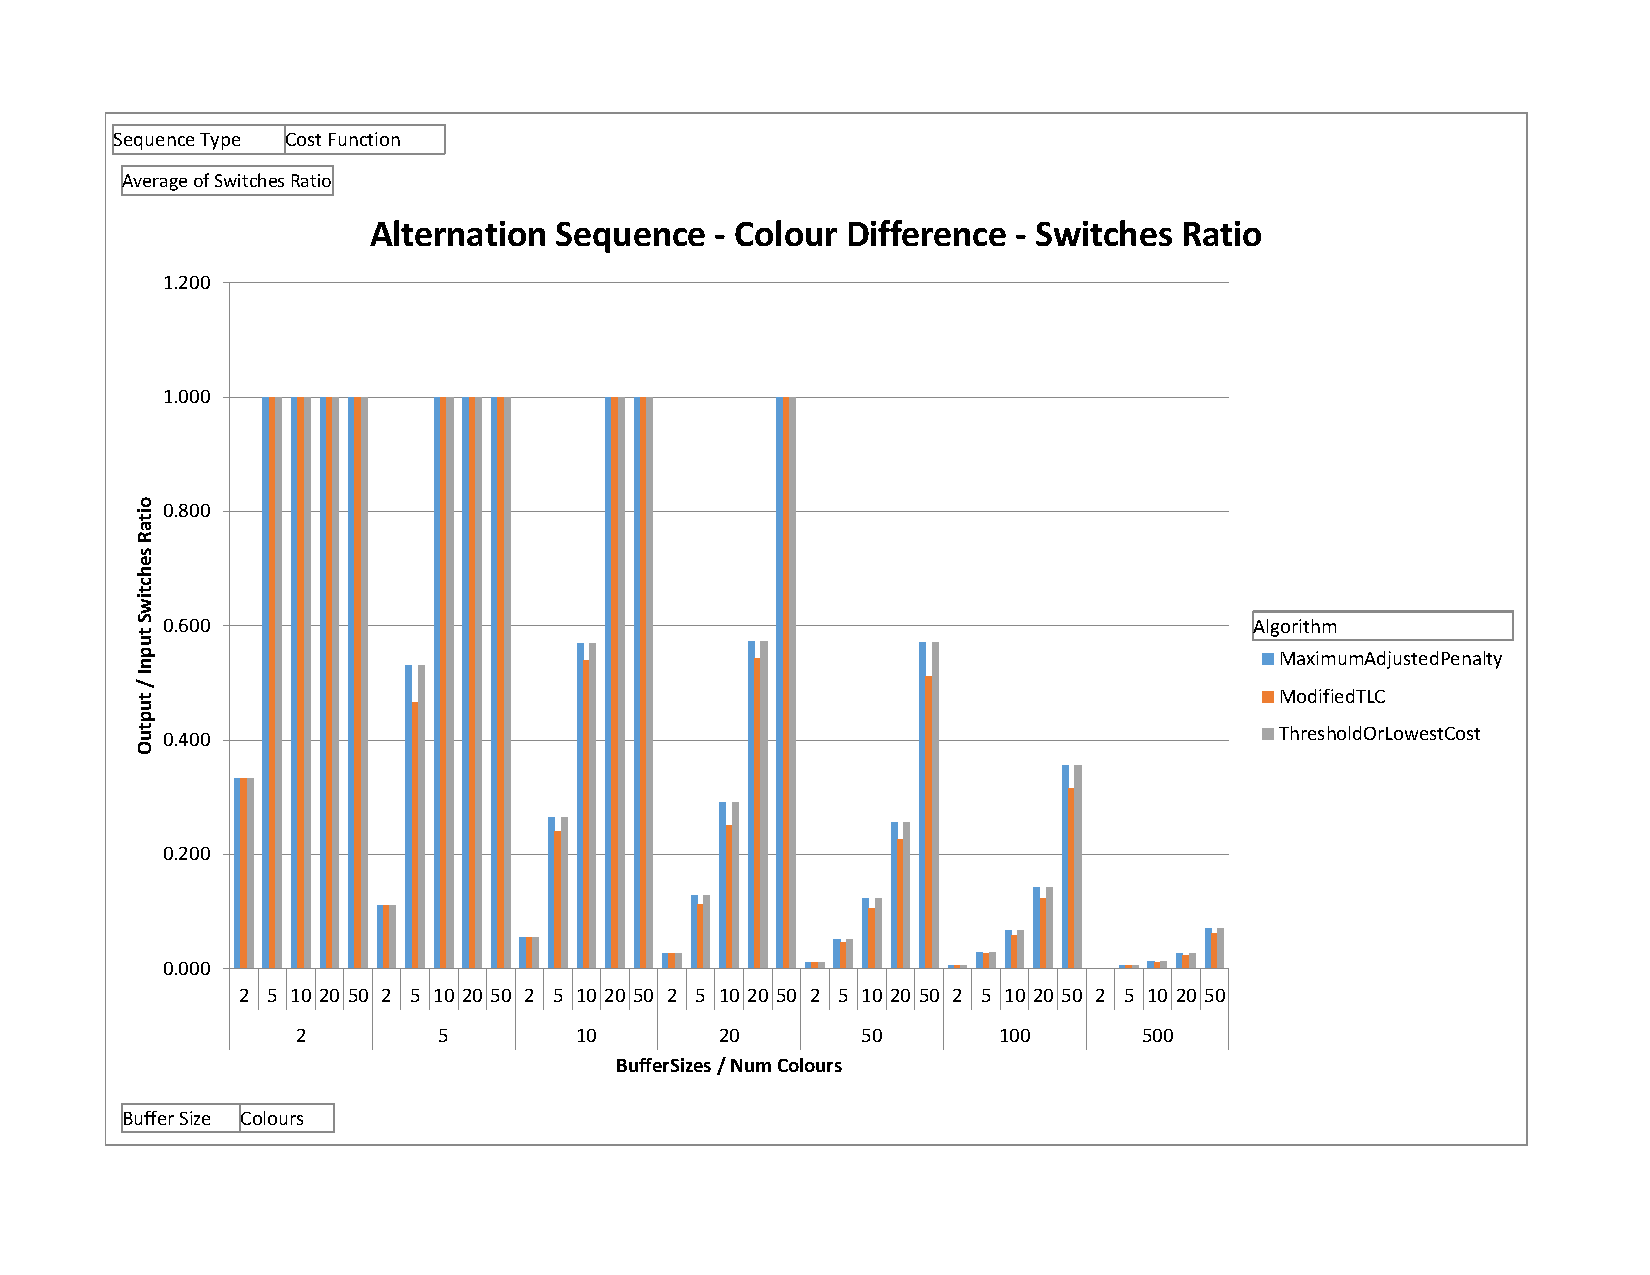
\includegraphics[scale=0.60]{Alternation-Seq-Colour-Difference-Switches.pdf}
\caption{Alternation-Sequence-Colour-Difference-Switches-Ratio: MAP and TLC have the exact same performance}
\label{AlternationSeqColourDifferenceSwitches}
\end{figure}

\subsection{Delta Sequences}

As in the case of Alternation Sequences, the Uniform Cost model shows little variation across most of our algorithms with the performance varying only marginally for all buffer sizes and colours. It is also interesting to note that as with alternation sequences, Random Choice is still the algorithm that has the highest cost, although this seems to be the case with larger buffers and many colours. 

For Delta Sequences with the Cost Equals Colour model, we find that TLC performs marginally well only for very small buffers with very few colours. MAP and ModifiedTLC outperform TLC by a very large margin for all other combinations of buffer sizes and number of colours. The variation between MAP and ModifiedTLC is marginal for most cases and when the number of colours is very small they are nearly the same. In the best case, with a buffer size of 500 and 50 colours, ModifiedTLC and MAP only have 5\% of the cost present in the input sequence.

ModifiedTLC and MAP perform significantly better than TLC for the Cost Equals Quadratic Cost model, with the performance getting better as the buffer size increases. For very small and very large buffer sizes ModifiedTLC performs marginally better than MAP, but MAP performs better than ModifiedTLC for medium sized buffers. This is illustrated in Figure \ref{DeltaSeqCostEqualsQuadraticColour}. 

\begin{figure}[ht]
\centering 
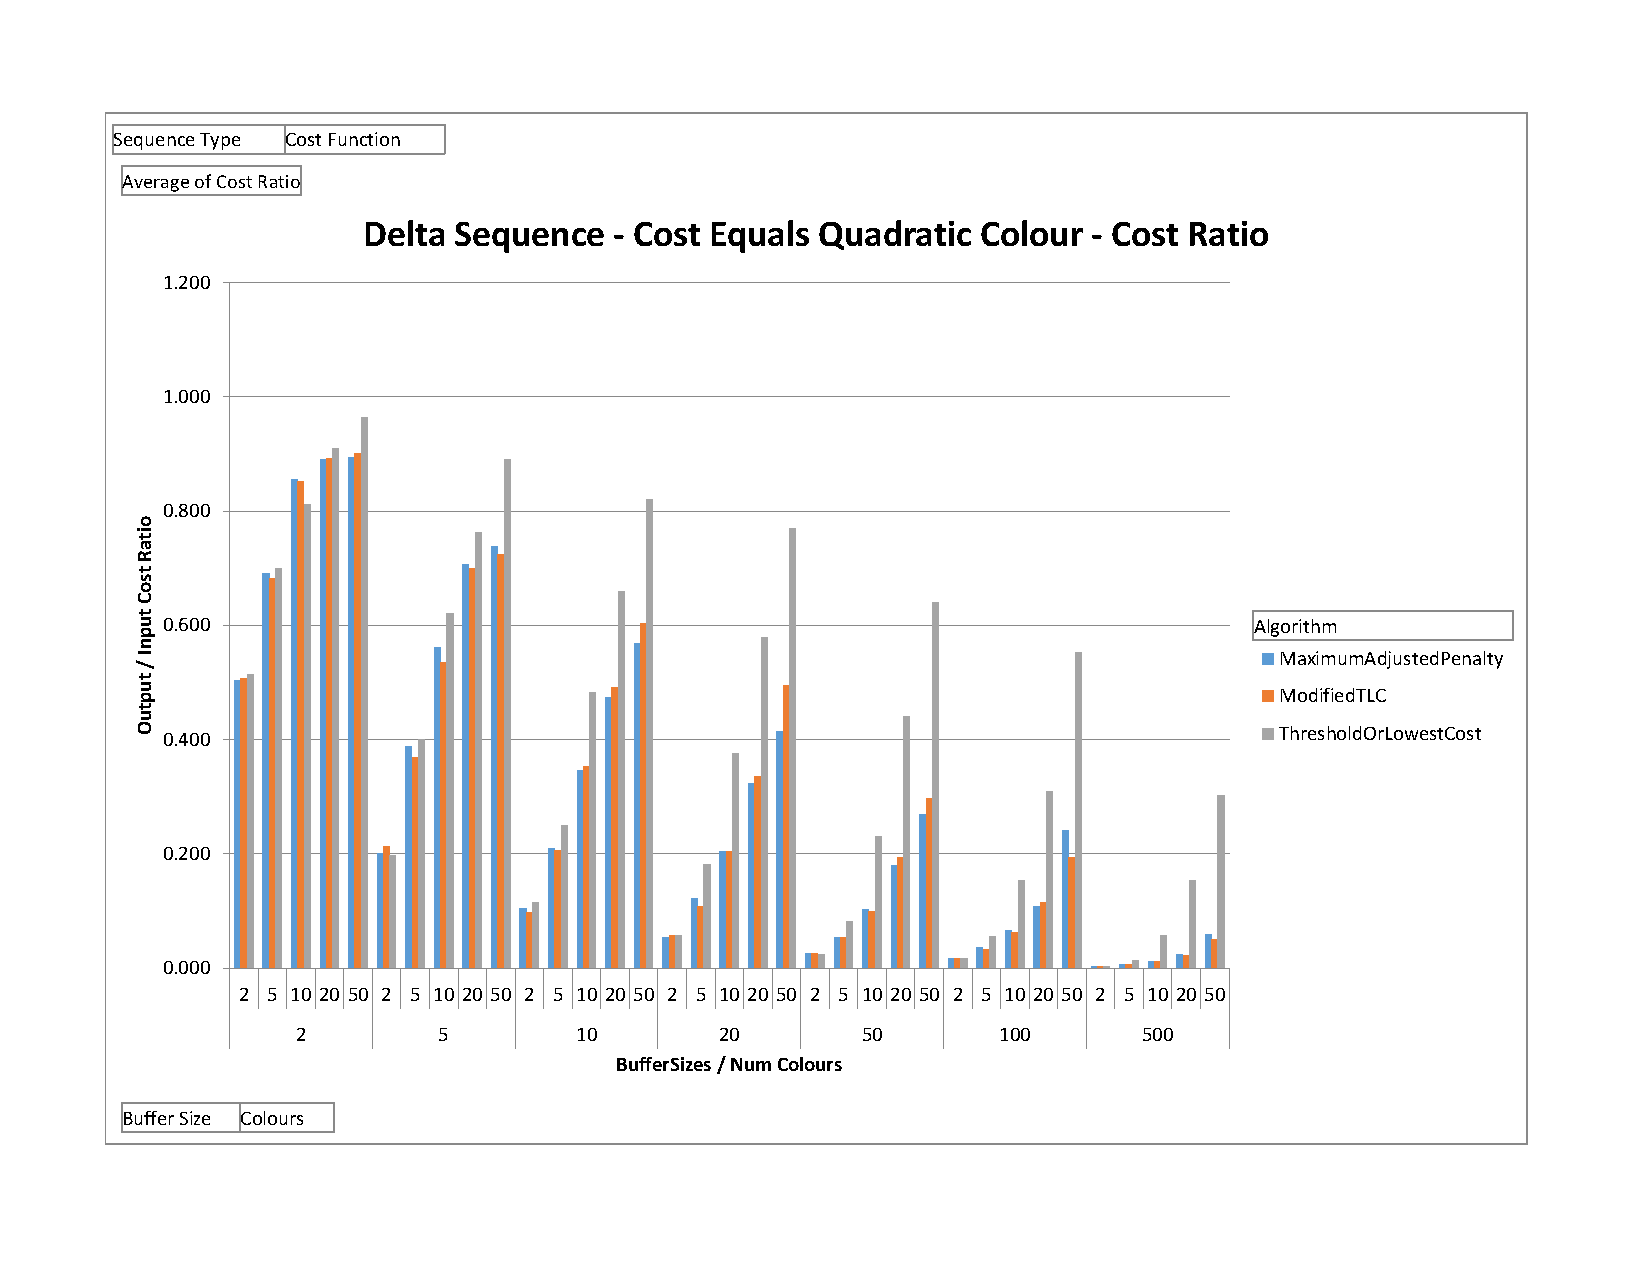
\includegraphics[scale=0.60]{Delta-Seq-Cost-Equals-Quadratic-Colour.pdf}
\caption{Delta-Sequence-Cost-Equals-Quadratic-Colour-Cost-Ratio: ModifiedTLC and MAP achieve better performance than TLC}
\label{DeltaSeqCostEqualsQuadraticColour}
\end{figure}

The performance trend continues with the Random Cost model with ModifiedTLC and MAP achieving significantly better performance than TLC across all buffer sizes and number of colours. It is also interesting to note that the variation between ModifiedTLC and MAP is marginal across all cases. For small buffers ModifiedTLC and MAP perform slightly better than TLC and the performance improvement improves as the buffer size increases. Another point of interest is that, ModifiedTLC and MAP greatly reduce the number of switches present in the input sequence, with ModifiedTLC doing slightly better than MAP. For very small number of colours, all algorithms achieve the same performance. These are illustrated in Figure \ref{DeltaSeqRandomCost}.

\begin{figure}[ht]
\centering 
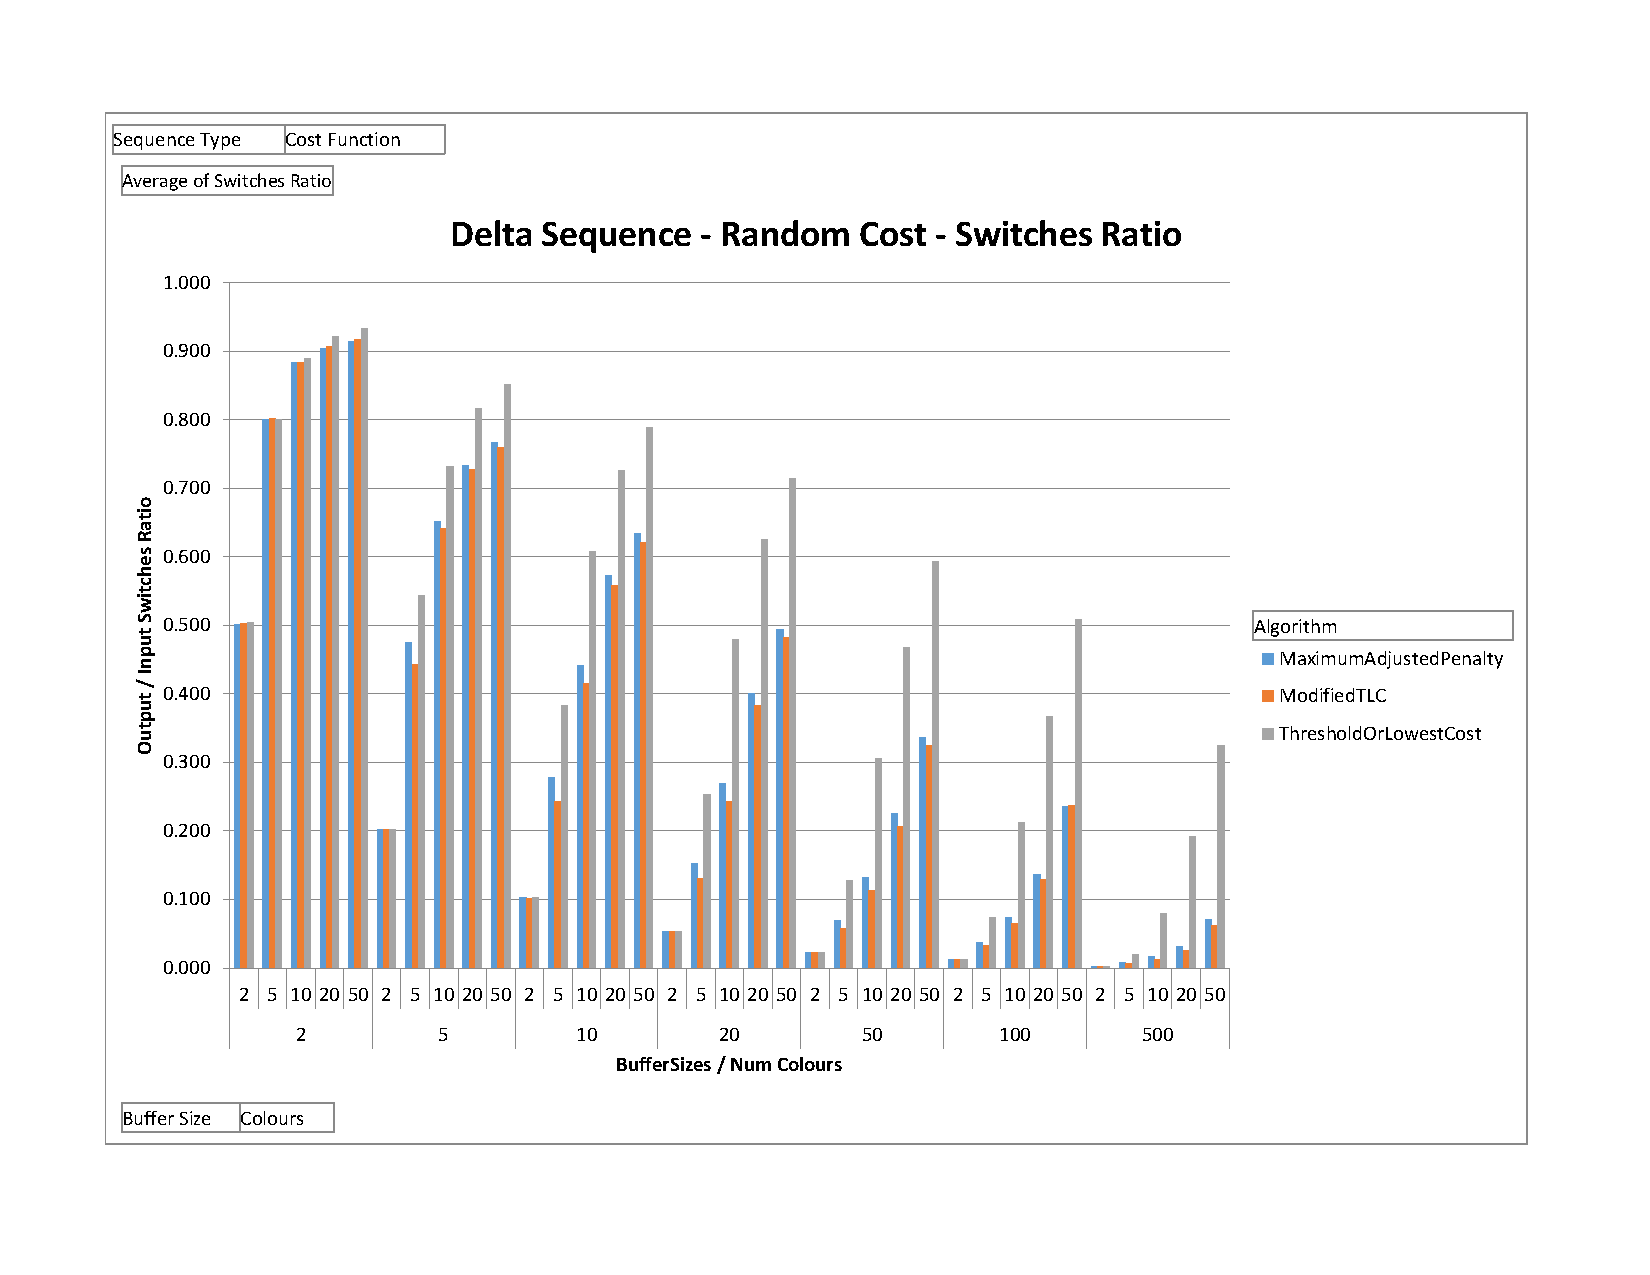
\includegraphics[scale=0.60]{Delta-Seq-Random-Cost-Switches.pdf}
\caption{Delta-Sequence-Random-Cost-Cost-Ratio: ModifiedTLC and MAP achieve better performance than TLC}
\label{DeltaSeqRandomCost}
\end{figure}

ModifiedTLC seems to perform poorly with the Colour Difference Cost model, however TLC achieves a good performance for this model across all buffer sizes and colours. Although, ModifiedTLC makes a performs slightly better than MAP and TLC when comparing the switch ratio, it seems to make expensive switches, which account for the higher cost ratio.

\subsection{Random Sequences}

While there is no one algorithm that achieves exceptional performance for the Uniform Cost model, Bounded Waste achieves a better performance among all algorithms. Random Choice achieves the worst performance among all our algorithms and the difference between the cost ratios among the others is marginal. 

For a buffer size of 2, TLC performs better than MAP and ModifiedTLC, however ModifiedTLC and MAP achieve significantly better performance in terms of both switch and cost ratios for all other buffer sizes and number of colours. This trend is also seen with the Cost Equals Colour Quadratic Cost model, with ModifiedTLC achieving a better switch ratio when compared to both MAP and TLC as illustrated in Figure \ref{RandomSeqCostEqualsColourQuadraticSwitches}. 

\begin{figure}[ht]
\centering 
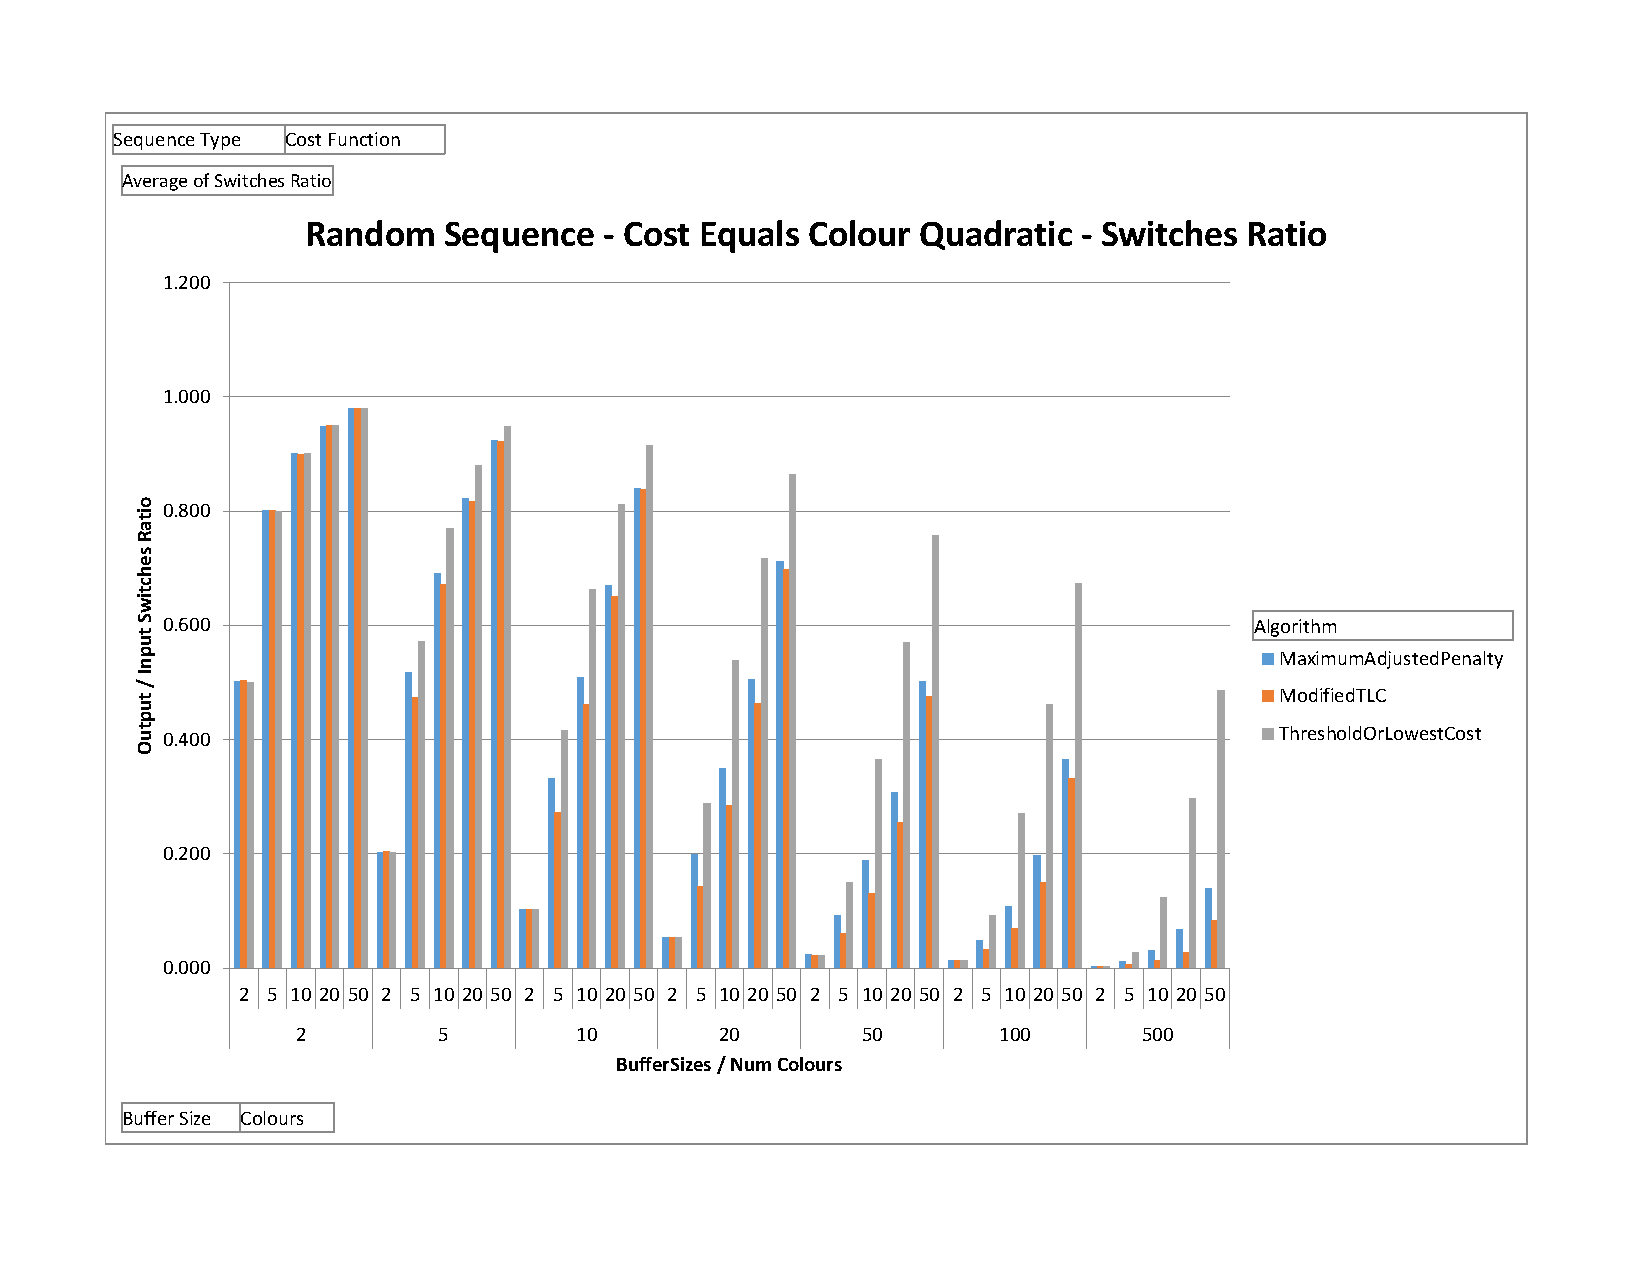
\includegraphics[scale=0.60]{Random-Sequence-Cost-Equals-Colour-Quadratic-Switches.pdf}
\caption{Random-Sequence-Cost-Equals-Colour-Quadratic-Switches-Ratio}
\label{RandomSeqCostEqualsColourQuadraticSwitches}
\end{figure}

ModifiedTLC is the algorithm of choice for Random Sequences with the Random Cost model as illustrated in Figure \ref{RandomSeqRandomCost}.  We observe that the performance of ModifiedTLC and MAP when compared to TLC improves significantly as the size of the buffer increases. 

\begin{figure}[ht]
\centering 
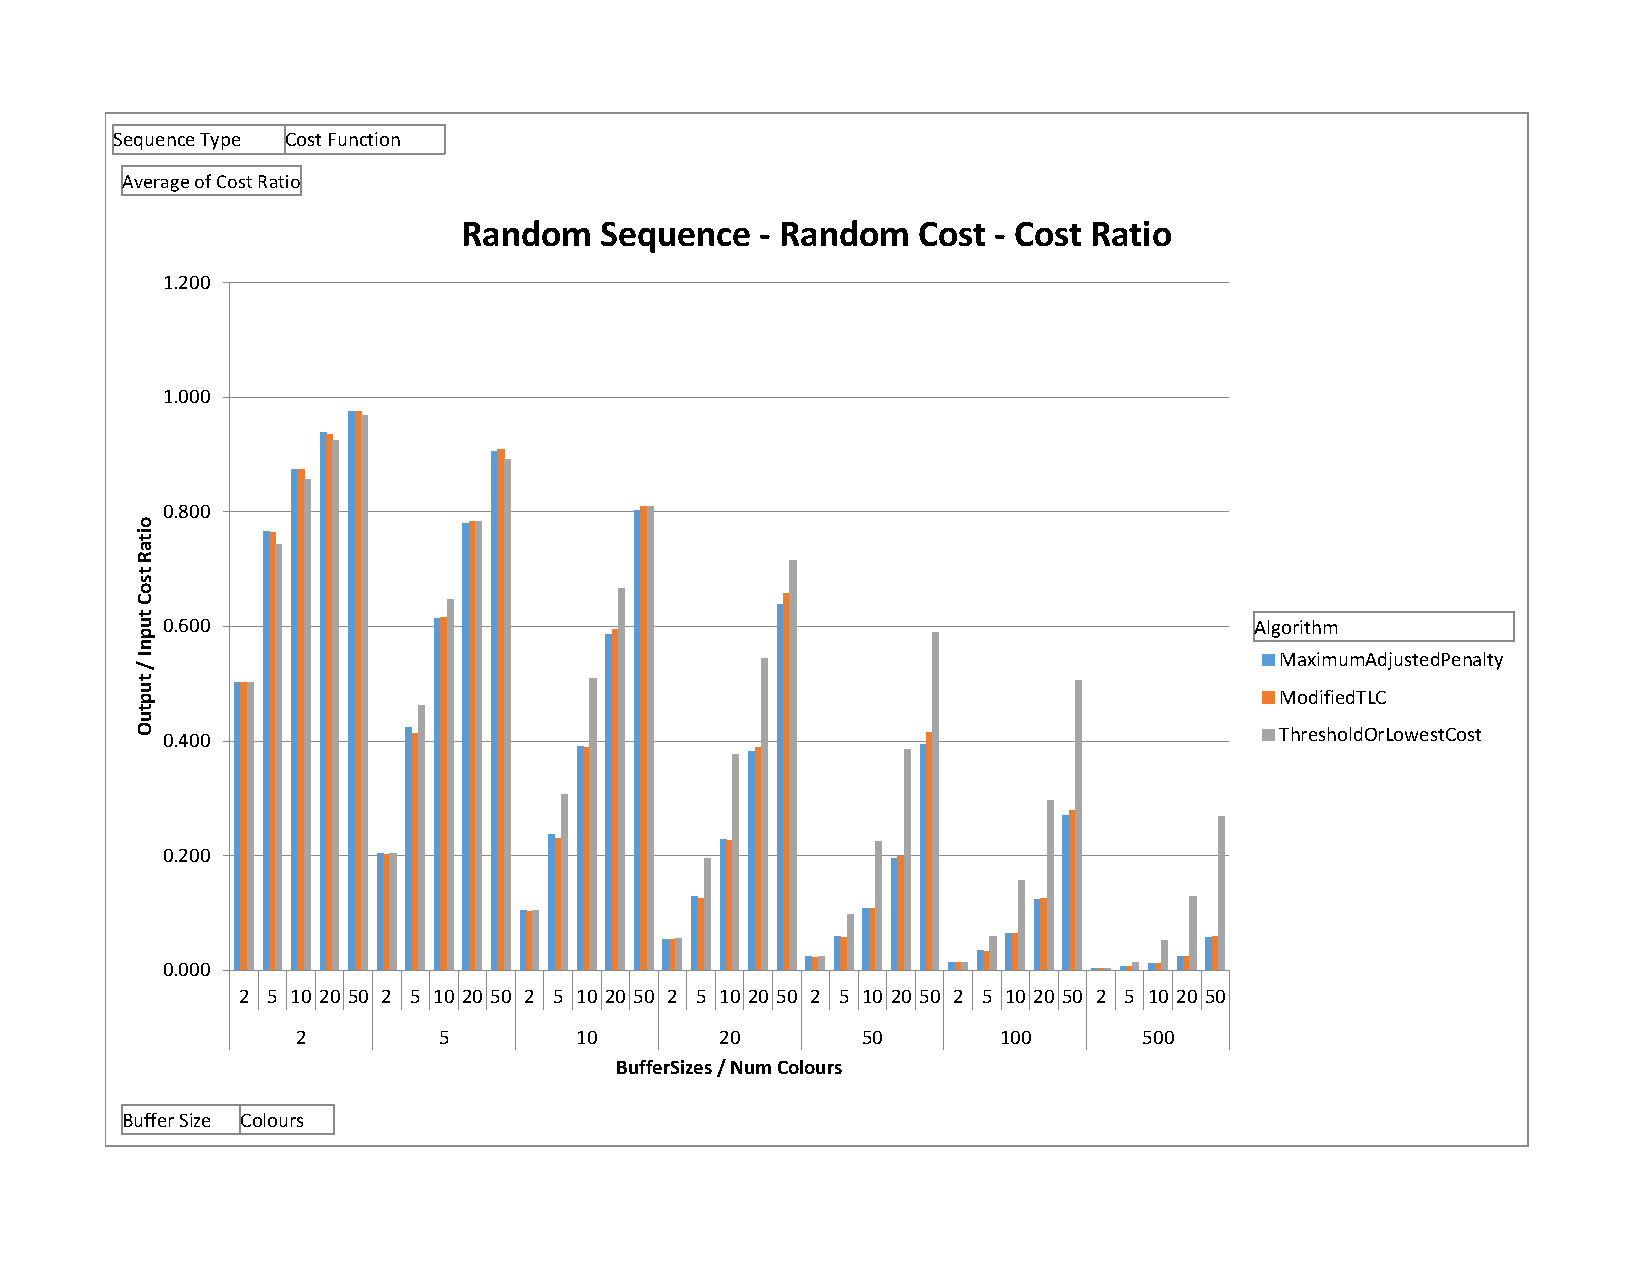
\includegraphics[scale=0.60]{Random-Seq-Random-Cost.pdf}
\caption{Random-Sequence-Random-Cost-Cost-Ratio}
\label{RandomSeqRandomCost}
\end{figure}

While ModifiedTLC achieves a marginally better switch ratio when compared to TLC and MAP, we observe that it performs poorly when cost ratios are compared. TLC achieves the best performance for the Colour Difference Cost Function in terms of reducing the cost incurred while switching between colours. 

\subsection{Random Block Sequences}

Random Block Sequences as expected do not achieve significant reordering because of the block nature of the input sequence. Uniform Cost model only has minimal reordering even with buffer sizes of 50 and 100. Of the algorithms, Bounded Waste achieves the best reordering in most cases, but overall, there is little reordering with this input sequence across all algorithms.

For the Cost Equals Colour cost model we observe that the cost ratios are almost identical for small buffer sizes (2 and 5), for larger buffer sizes, ModifiedTLC performs better than TLC and MAP both in terms of cost and switch ratios as illustrated in Figure \ref{RandomBlockCostEqualsColour}.

\begin{figure}[ht]
\centering 
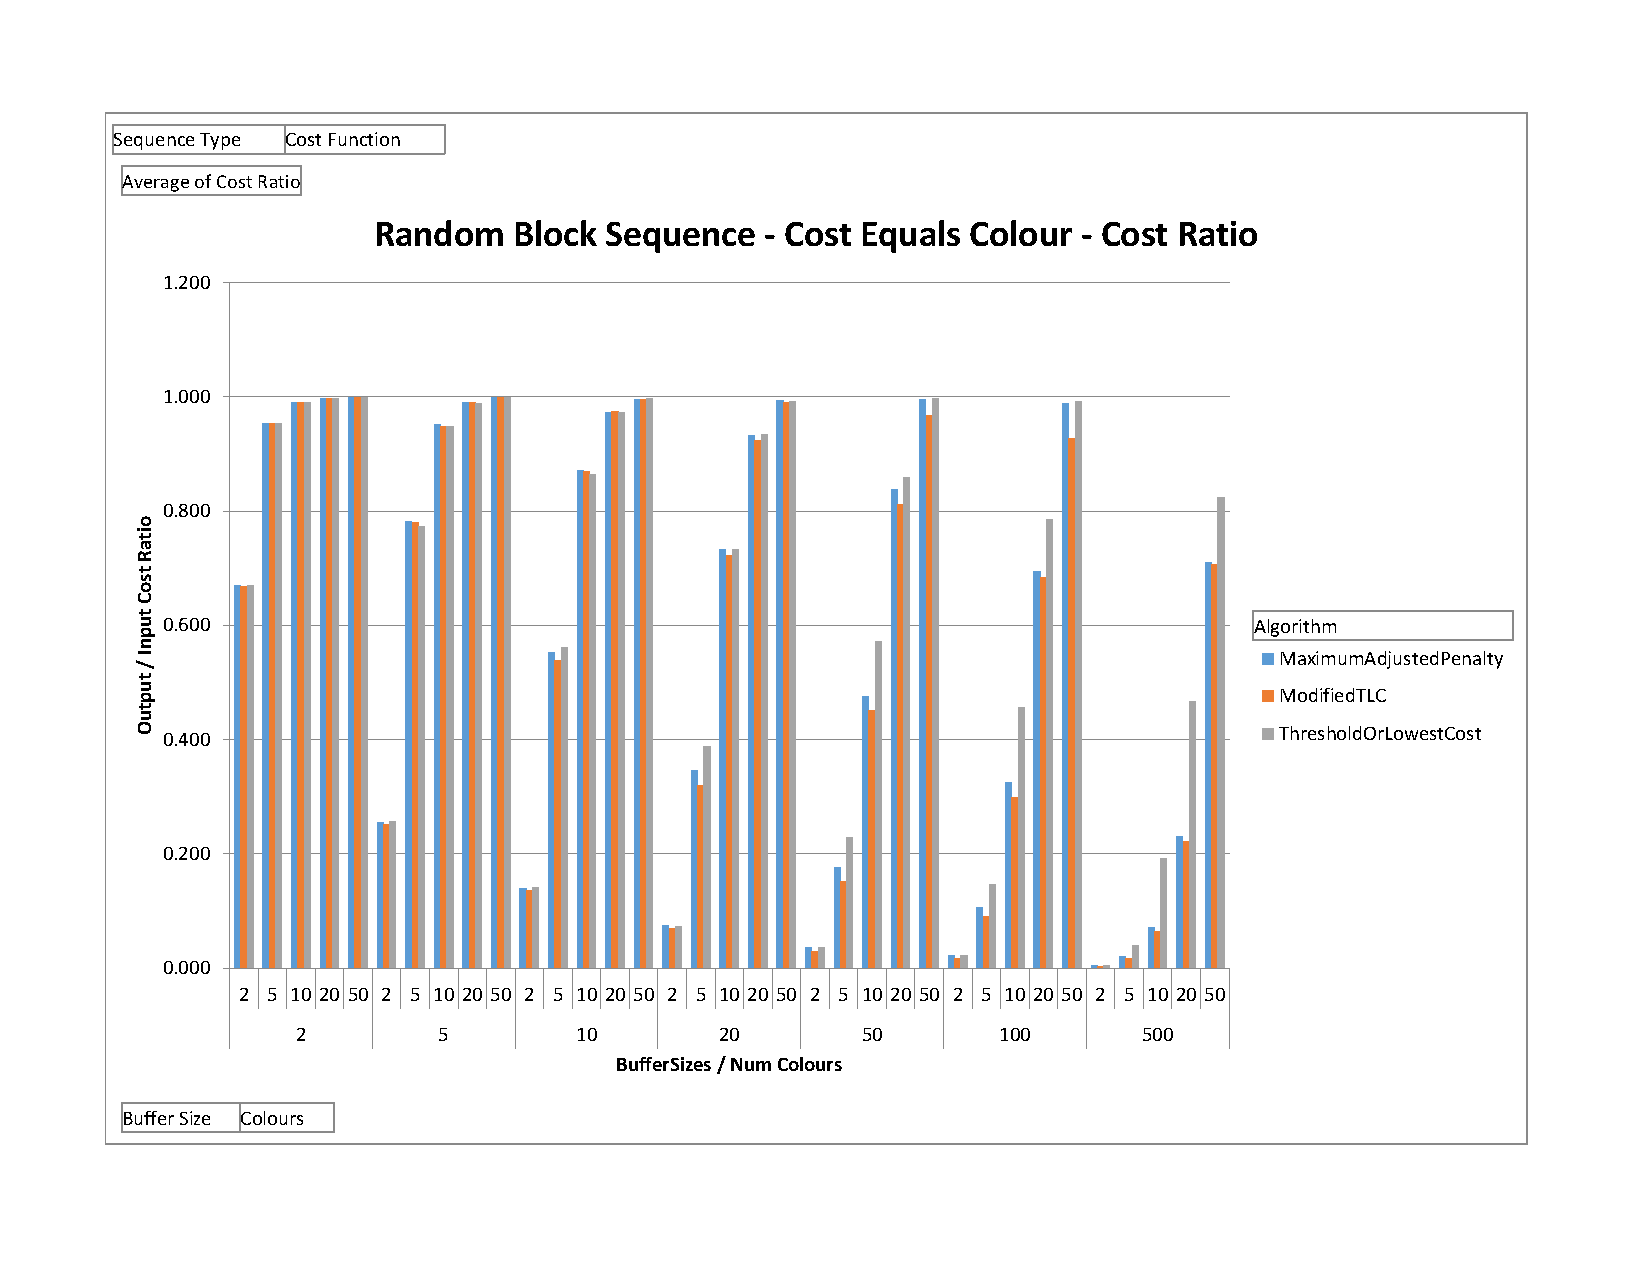
\includegraphics[scale=0.60]{Random-Block-Cost-Equals-Colour.pdf}
\caption{Random-Block-Cost-Equals-Colour-Cost-Ratio}
\label{RandomBlockCostEqualsColour}
\end{figure}

As expected, we only see minimal reordering for the Random Block input sequences, for very small buffer sizes and large number of colours. All our algorithms achieve similar switch ratios for very small buffer sizes (2 and 5). For larger buffer sizes, MAP and TLC achieve similar switch ratios, and ModifiedTLC performs slightly better than the two for all different combinations of buffer sizes and number of colours. However, when we compare the cost ratios for the different algorithms, we find that the ratios are extremely similar for between all algorithms across different buffer size and number of colour combinations. MAP performs marginally better than TLC and ModifiedTLC, although we have also noted that for buffer size 50, and 50 colours, MAP has a cost ratio of 1.034, which means that the output sequence has a cost which is 3.4\% more than the input sequence. This has been observed with the Cost Equals Colour Quadratic cost model. 

For Random Block sequences with the Random Cost model, all of our algorithms achieve similar performance for small buffer sizes. As the buffer size increases, we observe that ModifiedTLC and MAP perform better than TLC with ModifiedTLC having the best performance  as illustrated in Figure \ref{RandomBlockRandomCost}. 

\begin{figure}[ht]
\centering 
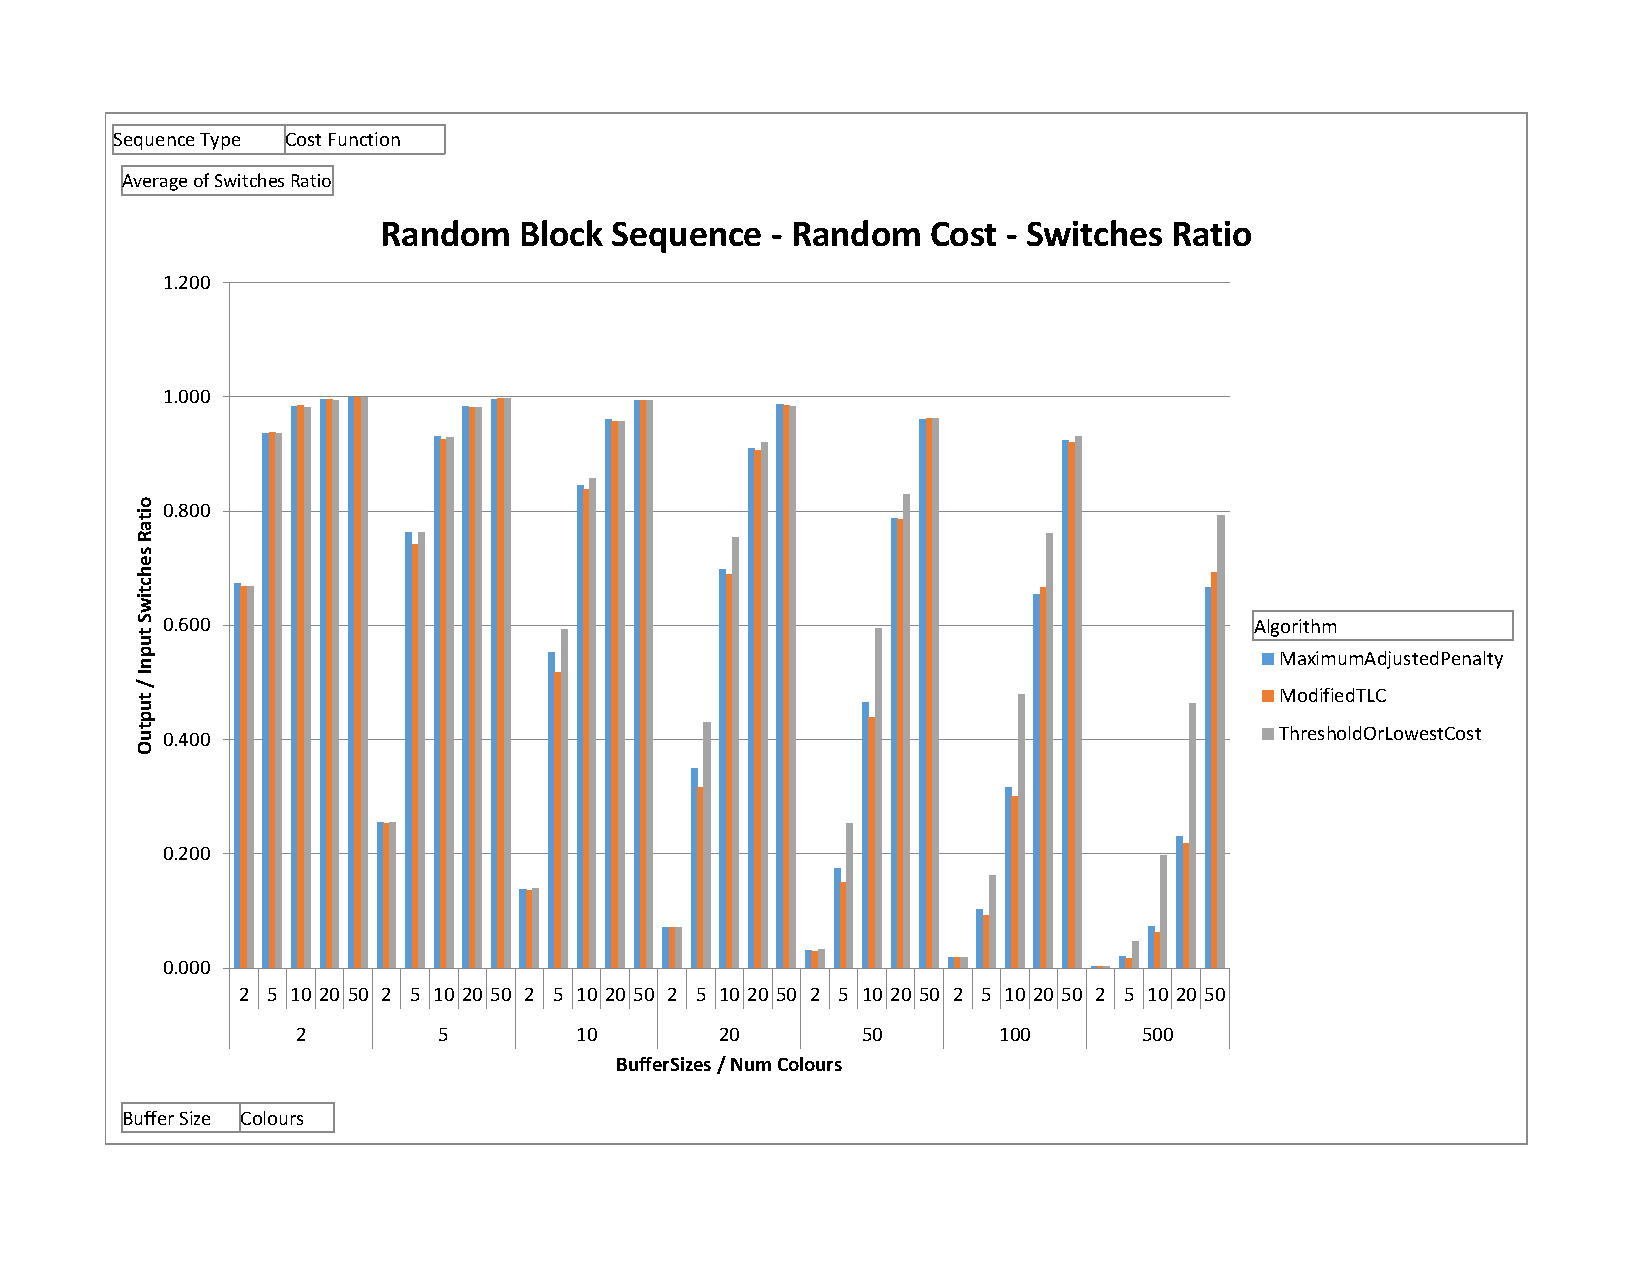
\includegraphics[scale=0.60]{Random-Block-Random-Cost-Switches.pdf}
\caption{Random-Block-Random-Cost-Switches-Ratio}
\label{RandomBlockRandomCost}
\end{figure}

MAP and TLC achieve a similar performance when it comes to the Colour Difference cost model, with TLC doing better than MAP when the cost ratios are compared. We observe that ModifiedTLC performs poorly when compared to MAP and TLC for the Colour Difference cost model. Hence TLC is the algorithm of choice for applications where the cost is a function of the difference between the colours concerned.

\subsection{Sequential Block Sequences}

Sequential Block Sequences achieve little or no reordering for the Uniform Cost model. For very small buffer sizes (2 and 5) the output sequence is identical to the input sequence across all the algorithms. This behaviour is expected since we have chosen our block size to be 5 and a buffer size of 2 or 5 would mean that the buffer can only see items of one block, forcing it to make a colour change at every block. For larger buffer sizes (10, 20, 50 and 100), we notice that Bounded Waste achieves a good performance followed by Round Robin and Random Choice. It is interesting to note that for a buffer size of 20 with 5 colours, Bounded Waste fails to reorder the input sequence while other algorithms achieve a better performance in that particular case. 

As in the case of Uniform Cost model, all algorithms fail to reorder the input sequence for the Cost Equals Colour Model for very small buffer sizes. TLC achieves a better performance than MAP and ModifiedTLC when for medium buffer sizes (10, 20, 50 and 100) when the number of colours are large. It is interesting to note that MAP and ModifiedTLC fail to reduce the cost of reordering in these cases making TLC the most suited algorithm for Sequential Block Sequences with the Cost Equals Colour model. However, it may be noted that for very large buffer sizes, ModifiedTLC and MAP reduce the switching cost significantly, since MAP is computationally intensive, ModifiedTLC would be the algorithm of choice in this case as illustrated in Figure \ref{SequentialBlockCostEqualsColour}. 

\begin{figure}[ht]
\centering 
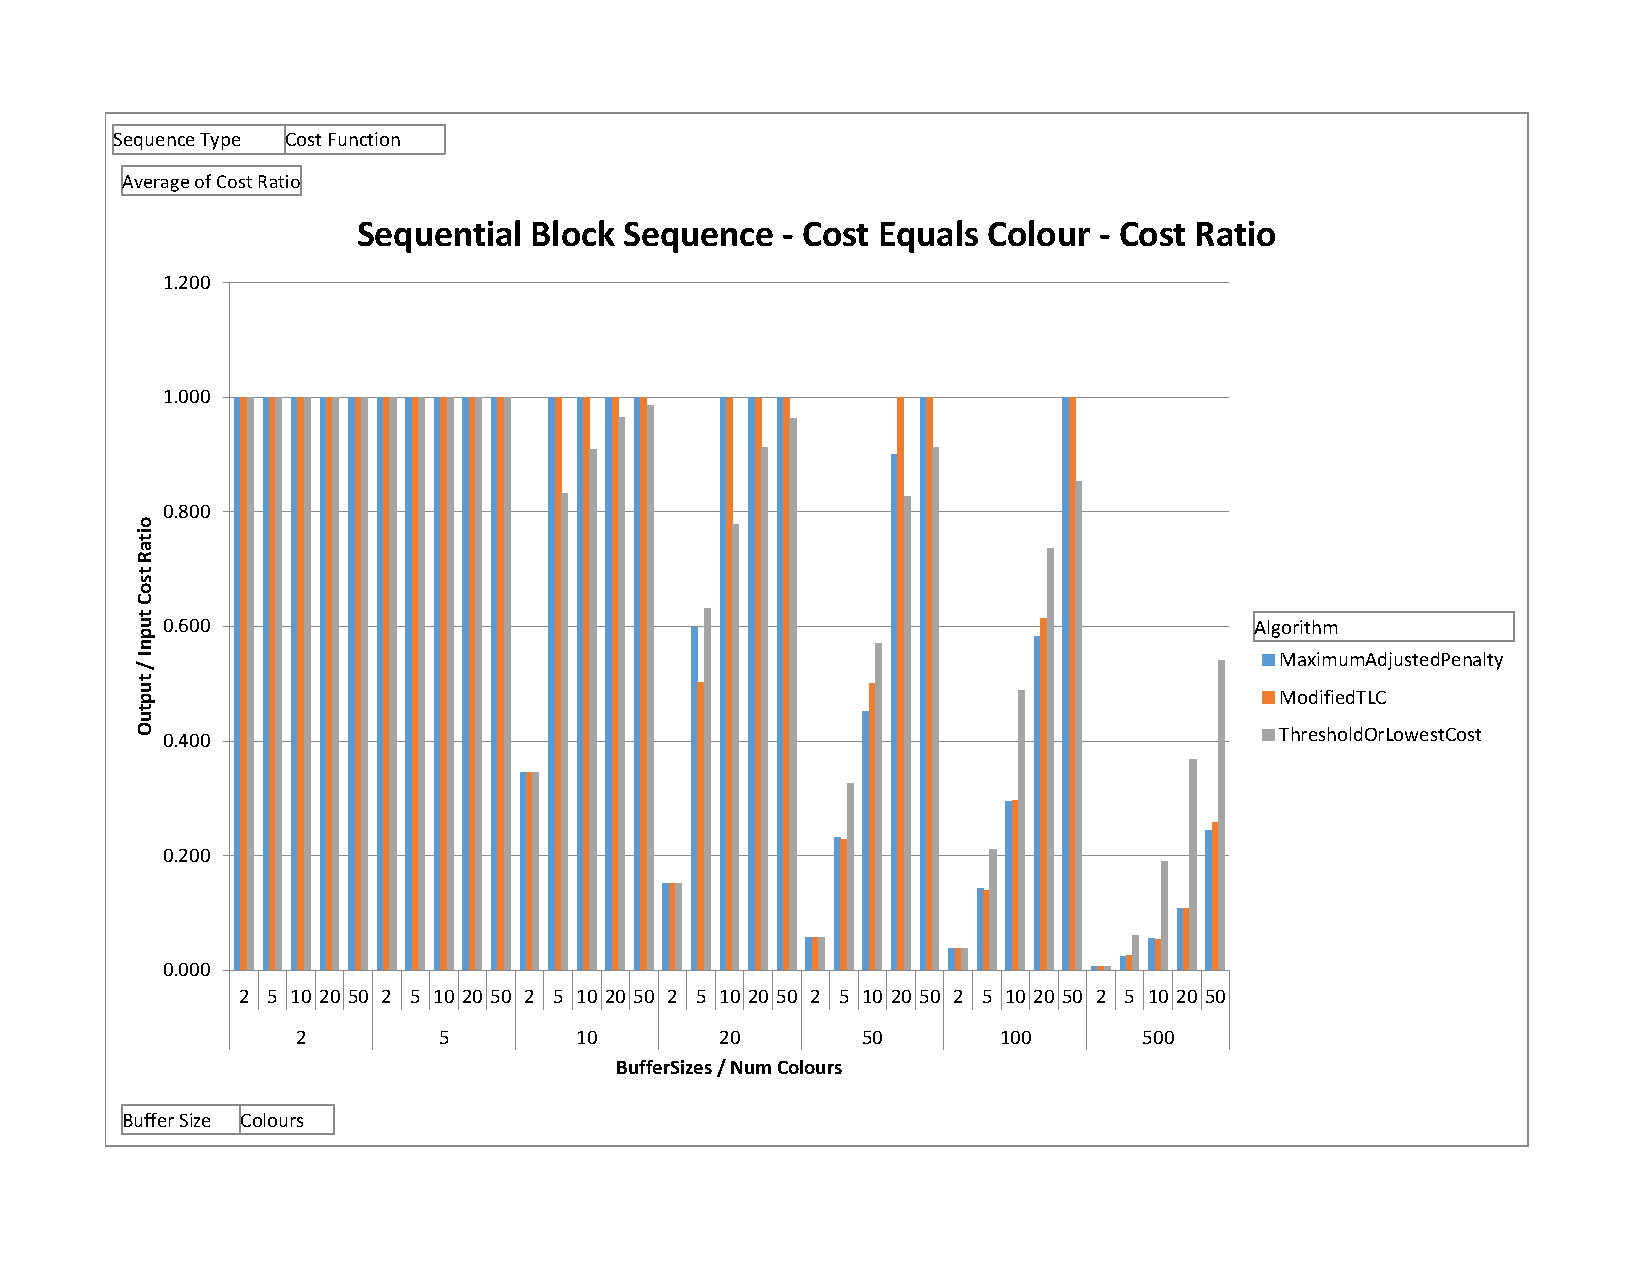
\includegraphics[scale=0.60]{Sequential-Block-Cost-Equals-Colour.pdf}
\caption{Sequential-Block-Cost-Equals-Colour-Cost-Ratio}
\label{SequentialBlockCostEqualsColour}
\end{figure}

Our algorithms follow a similar trend when it comes to the Cost Equals Colour Quadratic model, with no reordering observed for very small buffer sizes and TLC performing better than MAP and ModifiedTLC for medium sized buffers. However, as in the case of Cost Equals Colour model, MAP and ModifiedTLC perform significantly better than TLC for large buffers. While TLC does achieve a better reordering when compared to MAP and ModifiedTLC, the reordering is minimal owing to the nature of the sequence. 

For the Random Cost Model, ModifiedTLC achieves a better switch ratio when compared to TLC and MAP when the buffer size is larger than the number of colours as illustrated in Figure \ref{SequentialBlockRandomCostSwitches}. However, when comparing cost ration, all our algorithms have a few cases where the cost of reordering is higher than the cost incurred by the input sequence. This behaviour has been observed for buffer sizes 10, 20, 50 and 100, where the output cost is approximately 0.4\% higher than the input cost. 

\begin{figure}[ht]
\centering 
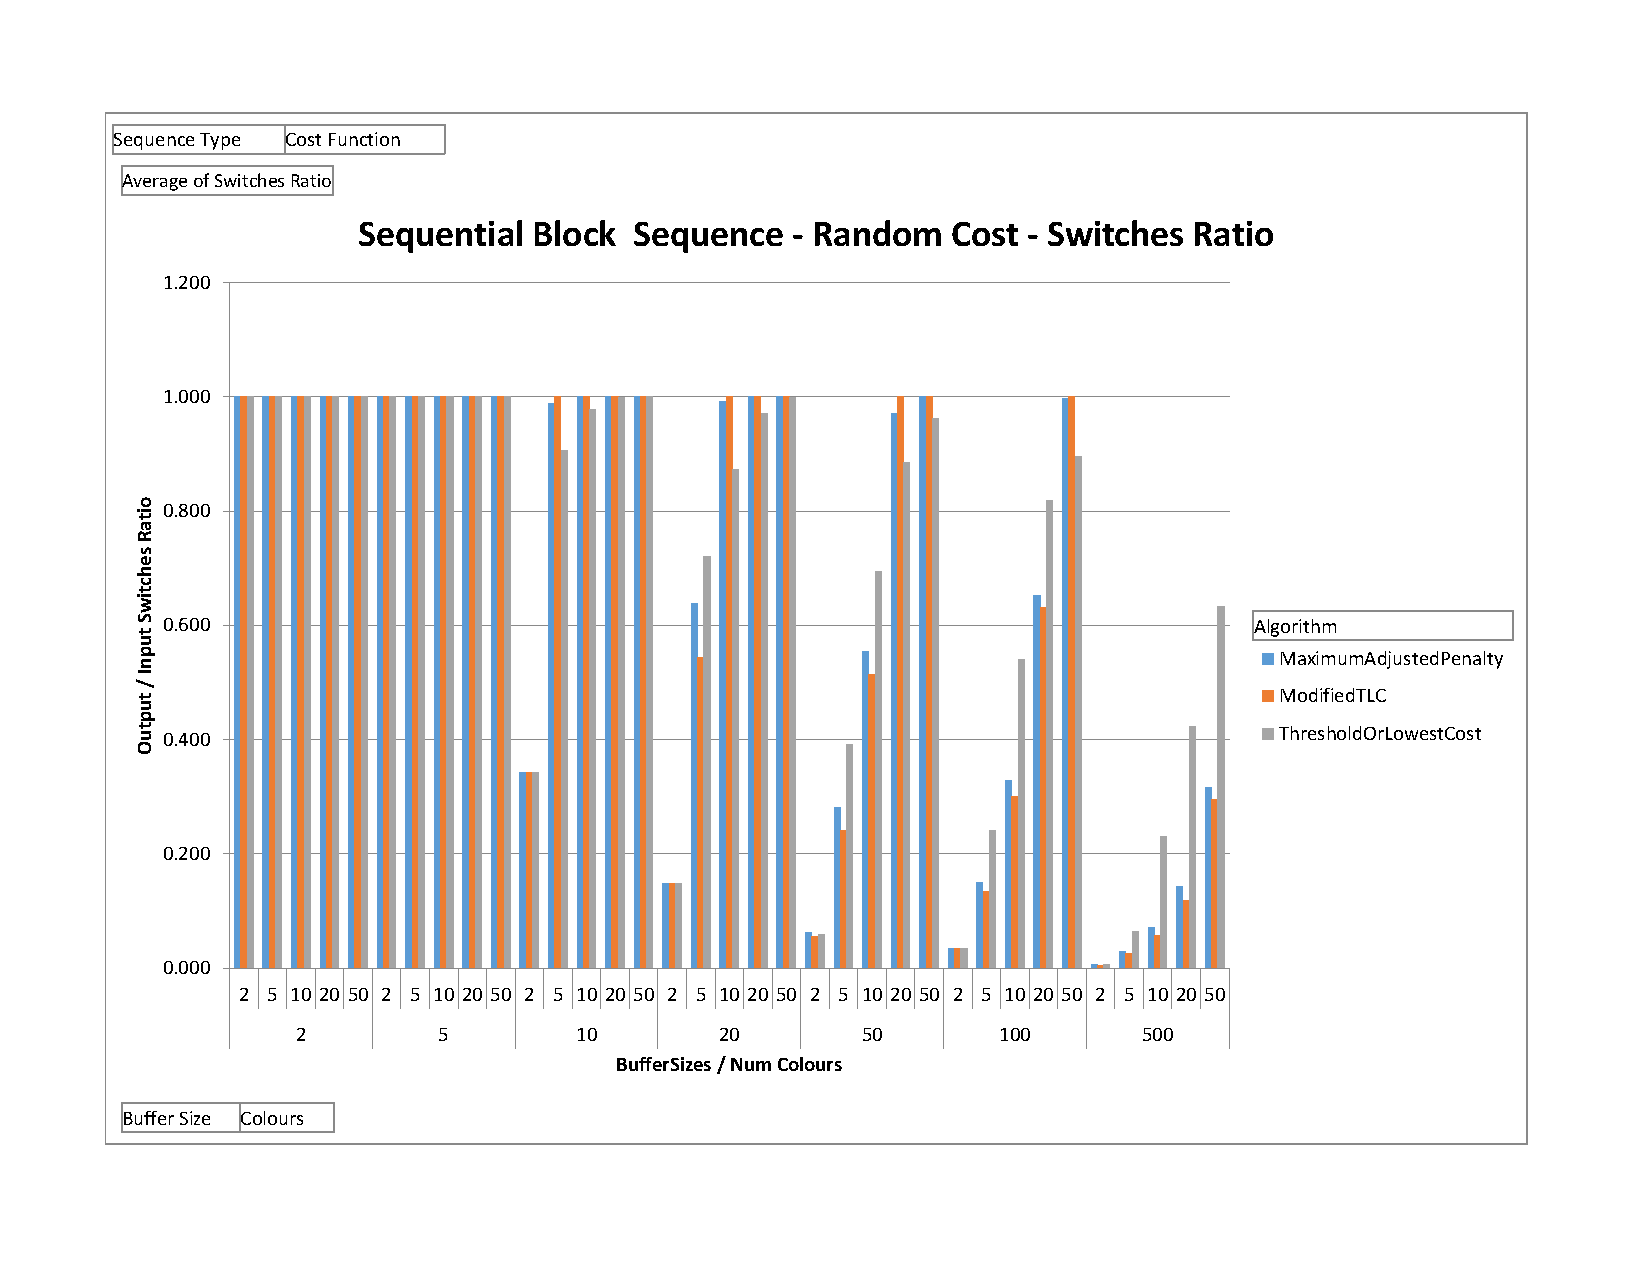
\includegraphics[scale=0.60]{Sequential-Block-Random-Cost-Switches.pdf}
\caption{Sequential-Block-Random-Cost-Switches-Ratio}
\label{SequentialBlockRandomCostSwitches}
\end{figure}

As far as the Sequential Block Sequence is concerned, we observe the worst reordering behaviour for the Cost Difference model where our algorithms fail to achieve a good cost ratio even for medium buffer sizes. It is also interesting to note that ModifiedTLC is the worst suited for this cost model when we compare the cost ratios. We observe that for buffer size 20 with 10, 20 and 50 colours, ModifiedTLC significantly increases the cost of reordering by an average of 23.66\% making it unsuitable for this cost model. It is also interesting to note that while the cost ratio is increased significantly, the switch ratio observed for ModifiedTLC is better than those for MAP and TLC, with MAP and TLC achieving almost identical switch ratios.  

We compare all our algorithms against the Optimal Offline Linear Programming Algorithm and measure competitive rations accordingly. Since the linear program is excessively time intensive for larger input sizes, we also test our algorithms for input size 100 along with buffer size 100, which emulates the offline setting of the algorithm in question.
